\documentclass{report}

\usepackage[english]{babel}
\usepackage{circuitikz}


\title{Strand displacement neural networks and RNA translators}
\author{Daniel Svane Nielsen}
\date{\today}
\begin{document}

  \maketitle

  \begin{abstract}
  The purpose of this project is to investigate a previously designed method of creating strand displacement neural networks, and combine them with RNA translation, for possible future use in general biosensors and molecular computers. The strand displacement neural network is created using a DNA motif called the seesaw gate. The seesaw gate requires some specific domains to function, so to use arbitrary sequences as input to the network, the sequences have to be translated. This report first goes through the theory of neural networks and strand displacement reactions, and later applies it for recreating the seesaw neural network. It is successfully shown that simple neural networks (perceptrons) can be trained to realize specific logic operations based on their truth tables, but with some limitations. The RNA translator was intended to be transcribed from a DNA template, and the displacement reactions tested using a fluorescent reporter. It was not possible to transcribe the RNA strands, so no succesful RNA translation is shown in this report.
  \end{abstract}


  \tableofcontents

  \chapter{Introduction}
  % !TEX root = ../main.tex
Logic circuits using DNA and RNA has many interesting applications in diagnostics and treatment. An example is cancer detection, where miRNA's can be used as biomarkers \cite{Peng2016}. These biomarkers can be used as inputs for logic circuits, which can be designed to activate fluorescence signals \cite{Seelig2006} or enzymes \cite{Engelen2016} when combinations of biomarkers are present or absent. For example, a circuit could be designed to activate when 2 unique miRNA's are present at the same time.

A different approach to building logic circuits is using neural networks. One of the advantages of this approach, is that large-scale networks does not have to be designed by someone with knowledge of logic gates and circuitry. The inputs of the circuit simply have to be defined along with the required output, and the neural network can be trained to give the desired functionality.

The neural network approach to strand displacement circuits has already been developed by Qian et all in 2011 \cite{Qian2011}. The design is based on the seesaw gate motif, which requires that the inputs to the network must have very specific sequences. To use custom input sequences, like the miRNAs from cancer cells, the sequences have to be translated. This has also already been done, using two linked strand displacement reactions \cite{Picuri2009}.

This project is split into two parts.

The first part aims to lay out the groundwork for a software where the miRNAs one wishes to detect can be entered. The strands and concentrations required for a neural network that implements a desired truth table is then calculated, and could be readily ordered and used as a biosensor.

The second part aims to translate one RNA sequence into another RNA sequence, and measuring the outcome by a fluorescent reporter. This is almost identical to the experiment in Picuri et al 2009 \cite{Picuri2009}, but using RNA instead of DNA in the translation reactions. This is mostly done to show that the translators could also use RNA, but also to get some experience in a laboratory.

  %
  %% !TEX root = ../main.tex
\section{Logic gates}
Logic gates in electric circuits are usually made using transistors. They can take boolean inputs (0 or 1) and output another boolean signal depending on the inputs and type of logic gate. An example of an AND logic gate can be seen in figure \ref{and_gate}.

\begin{figure}[H]
\centering
\begin{tabular}{cccc}
    \begin{circuitikz}[baseline=-0.7ex]
        \draw (0,0) node[and port] (and1) {}
        (and1.in 1) [anchor=east] node {A}
        (and1.in 2) [anchor=east] node {B}
        (and1.out) [anchor=west] node {O};
    \end{circuitikz}
    &
    $\begin{array}{ccc}
        A & B & O \\ \hline
        0 & 0 & 0 \\
        0 & 1 & 0 \\
        1 & 0 & 0 \\
        1 & 1 & 1 \\
    \end{array}$
\end{tabular}

\label{and_gate}
\caption{To the left, an AND gate with inputs A and B, and output O. To the right, the truth table for the AND gate.}
\end{figure}

Different gates exist, with different truth tables. These gates can be combined into more complex circuits, like calculators and integrated circuits, which exist in all modern computers.



  \chapter{Theory}
  % !TEX root = ../main.tex
\section{Strand displacement}

  % !TEX root = ../main.tex
\section{Neural networks}
\subsection{In silico neural networks}
Artificial neural networks (referred to just as neural networks) is a software implementation of the connection of neurons in the brain. In computer science they have been used to solve a wide variety of problems, like character and facial recognition. They present an advantage over conventional programmatic methods, as they don't need explicit coding for each new problem \cite{Tu1996}. The simplest instance of neural networks is the single neuron, also known as the perceptron \cite{Lippmann} (perceptron and neuron is used interchangeably in this report). The perceptron can be used for simple decision making (giving yes/no answers) from a set of inputs. The logical 2-input AND operator is an example of a problem that can be solved with the perceptron \cite{ZhaoYanling}, where the perceptron can output 1 if both the inputs are 1, otherwise 0.

The perceptron works by taking all the inputs, and multiplying each input by its associated weight. If the sum of the multiplied inputs exceeds a certain threshold, the perceptron will output 1, otherwise 0. This is shown schematically in \fref{perceptron}.

\begin{figure}[h]
\includegraphics[width=\textwidth]{figures/perceptron.tikz}
\caption{Diagram of the artificial perceptron.}
\label{perceptron}
\end{figure}

The representation can be simplified to the type shown in \fref{perceptron_simple}. The weights and thresholds for the perceptron version of the 2-input AND gate can also be seen in \fref{perceptron_simple}.

\begin{figure}[h]
  \begin{subfigure}[t]{.49\textwidth}
    \includegraphics[width=\textwidth]{figures/perceptron_simple.tikz}
    \caption{}
    \label{perceptron_simple_a}
  \end{subfigure}
  \quad
  \begin{subfigure}[t]{.49\textwidth}
    \includegraphics[width=\textwidth]{figures/perceptron_and.tikz}
    \caption{}
    \label{perceptron_simple_b}
  \end{subfigure}
  \caption{\subref{perceptron_simple_a} Simple representation of a 2-input perceptron. \subref{perceptron_simple_b} Weights and thresholds on a perceptron that implements the 2-input AND gate.}
  \label{perceptron_simple}
\end{figure}

The perceptron is limited to classifying inputs that are linearly separable \cite{ZhaoYanling}, which rules out the XOR operation.


% \begin{figure}[H]
% \centering
% 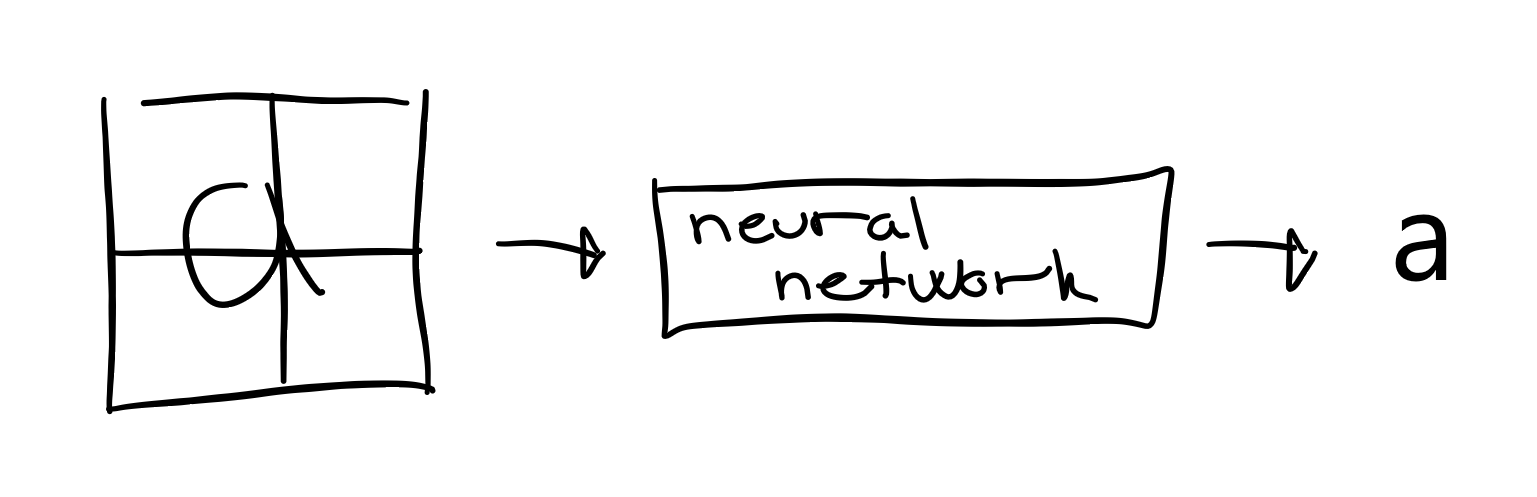
\includegraphics[width=\columnwidth]{images/neuralnetwork_example.png}
% \caption{An example usage of a neural network recognizing the handdrawn letter "a". The typical approach is to segment the area into a grid. Only 2x2 is shown here for simplification, but usually larger grids are used. The average color of each segment is calculated, and fed into a neural network, which has been trained to output "a", when presented an input resembling the handdrawn version.}
% \label{neuralnetwork_example}
% \end{figure}

% The neural network works by simulating the functionality of the brain, by connecting neurons together by varying strength. Continuing the example from figure \ref{neuralnetwork_example}, the 4 segments are fed into 4 input neurons (see figure \ref{neuralnetwork_neurons}). The 4 input neurons are connected to an output neuron by varying strength, much like the synapses of the natural neuron. If the weighted inputs sum exceed the threshold of the output neuron, it will activate. In this simplified example, the output neurons activation is of limited value, as it can only give a yes or no answer to if the input resembles an "a".

% \begin{figure}[H]
% \centering
% 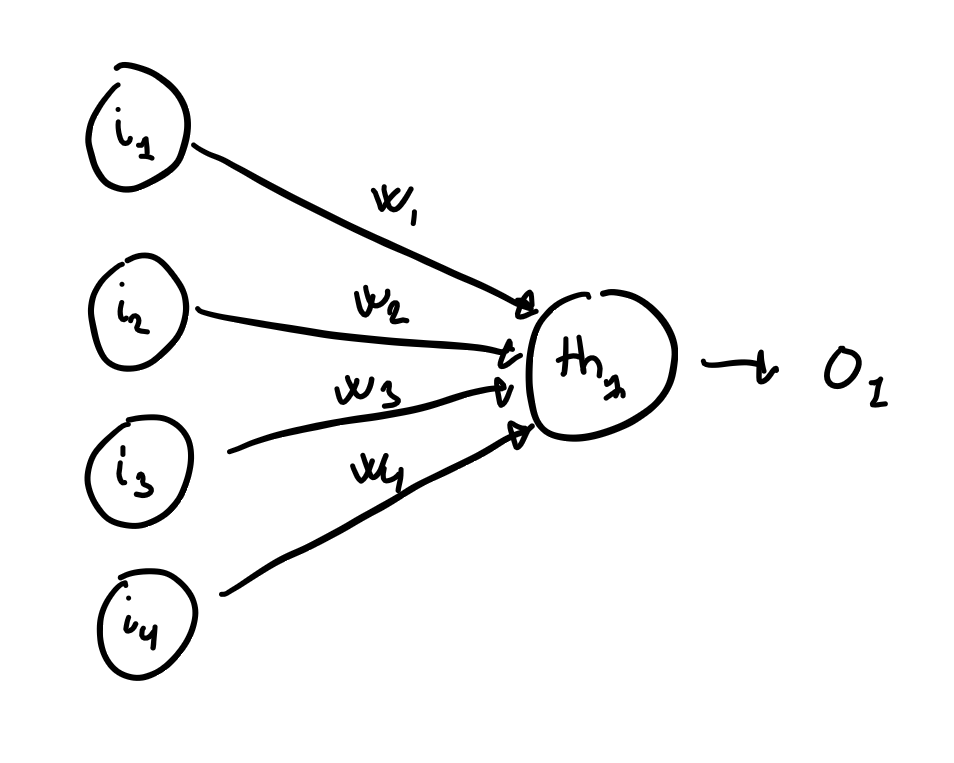
\includegraphics[width=200]{images/neuralnetwork_neurons.png}
% \caption{}
% \label{neuralnetwork_neurons}
% \end{figure}
%
%  In a more practical example, the network would have enough input neurons to accommodate a 100x100 grid (10,000 input neurons), have some layers of neurons between the input and output (hidden layers), and enough output neurons to represent binary encoded characters (see figure \ref{neuralnetwork_ocr}).
%
%  \begin{figure}[H]
%  \centering
%  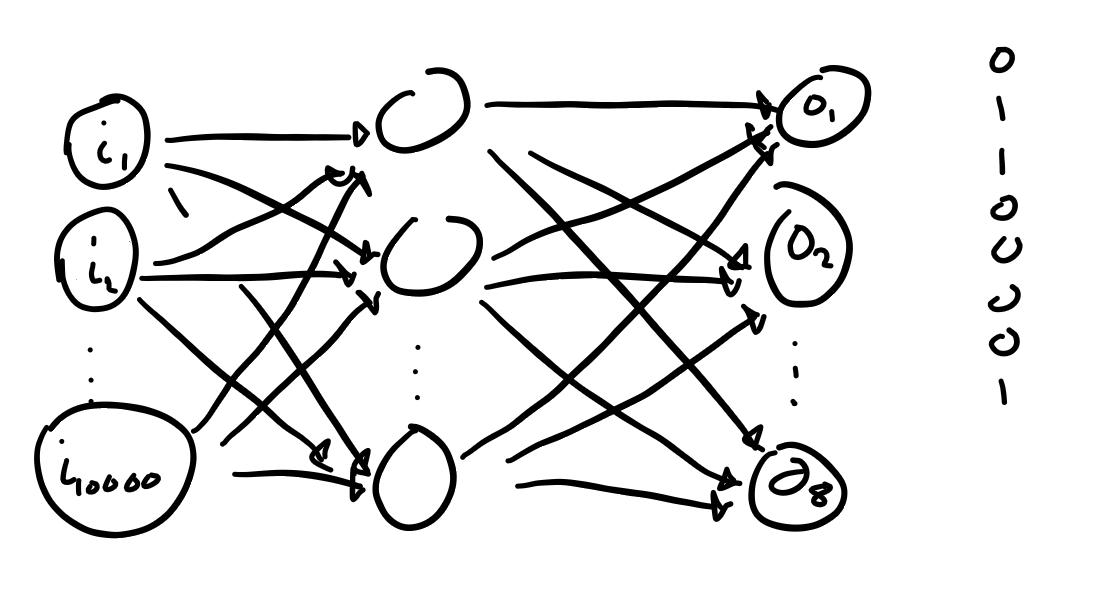
\includegraphics[width=\columnwidth]{images/neuralnetwork_ocr.png}
%  \caption{}
%  \label{neuralnetwork_ocr}
%  \end{figure}

\subsection{In vitro perceptron}
It has previously been shown that the function of the artificial neuron can also be implemented using strand displacement reactions. The system is based on the seesaw gate motif \cite{Qian}, and can fulfill most of the functionality of a real neuron \cite{Qian2011}. The seesaw gate is a catalytic gate with a threshold, designed for use in scalable strand displacement circuits. The seesaw gate uses a toehold to accelerate reactions, and has a left and right recognition domain to connect to other seesaw gates. The seesaw is named after the back and forth reaction of the strand displacement reactions, seen in \fref{seesaw}.

\begin{figure}[h]
\includegraphics[width=\textwidth]{figures/seesaw.tikz}
\caption{The back on forth reactions of the seesaw gate.}
\label{seesaw}
\end{figure}

The reaction can be pushed to the right by using a fuel strand, or the input can be reduced by using a threshold gate, the details of which are discussed below.

\subsubsection{Thresholding}
In the artificial neuron, the neuron will activate when its inputs exceeds a threshold. This is implemented using a threshold gate which will bind the input and prevent it from reacting downstream in the network. If the threshold gate concentration is higher than the input concentration, the input will be suppressed by the threshold. If the threshold gate concentration is lower than the input concentration, not all of the input is suppressed, and will be able to react further downstream in the network. This reaction is shown in \fref{seesaw_thresholding_reaction}.


\begin{figure}[h]
  \begin{subfigure}[t]{.49\textwidth}
    \includegraphics[width=\textwidth]{figures/seesaw_thresholding.tikz}
\caption{}
\label{seesaw_thresholding_reaction}
\end{subfigure}
\hfill
\begin{subfigure}[t]{.49\columnwidth}
  \centering
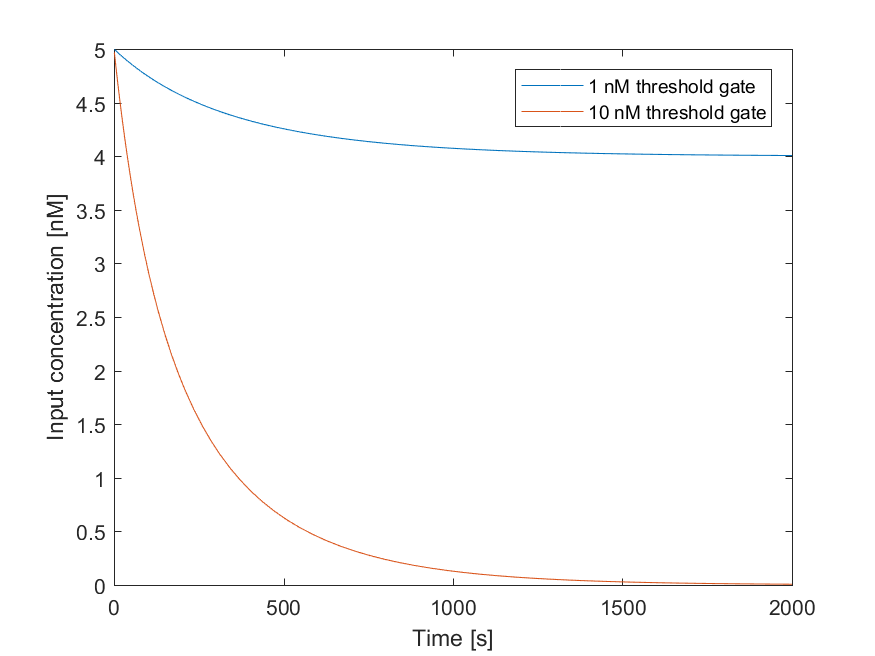
\includegraphics[width=\linewidth]{images/thresholding}

\caption{}
\label{seesaw_thresholding_analysis}
\end{subfigure}
\caption{\subref{seesaw_thresholding_reaction} Reaction of an input strand with a threshold gate. The product has no free toehold domain, and can't undergo reverse reaction. The waste has no toehold, and can't parcitipate in further reactions. \subref{seesaw_thresholding_analysis} Time analysis of the concentration of input strand (5 nM start concentration). A threshold concentration higher than the input (red) will bind all input strand. A lower concentration (blue), will allow the input strand to participate in further displacement reactions.}
\end{figure}

\subsubsection{Integration}
If the seesaw neuron have multiple inputs, they will have to be "collected" before thresholding, as they don't have the same left recognition sequence (see \fref{seesaw}). This is done through an integrating gate, which will collect all inputs with the same right recognition sequence, and release a common signal which can be thresholded. The integration gate is seen in \fref{seesaw_integration_reaction}.

\begin{figure}[h]
\begin{subfigure}[t]{.49\textwidth}
  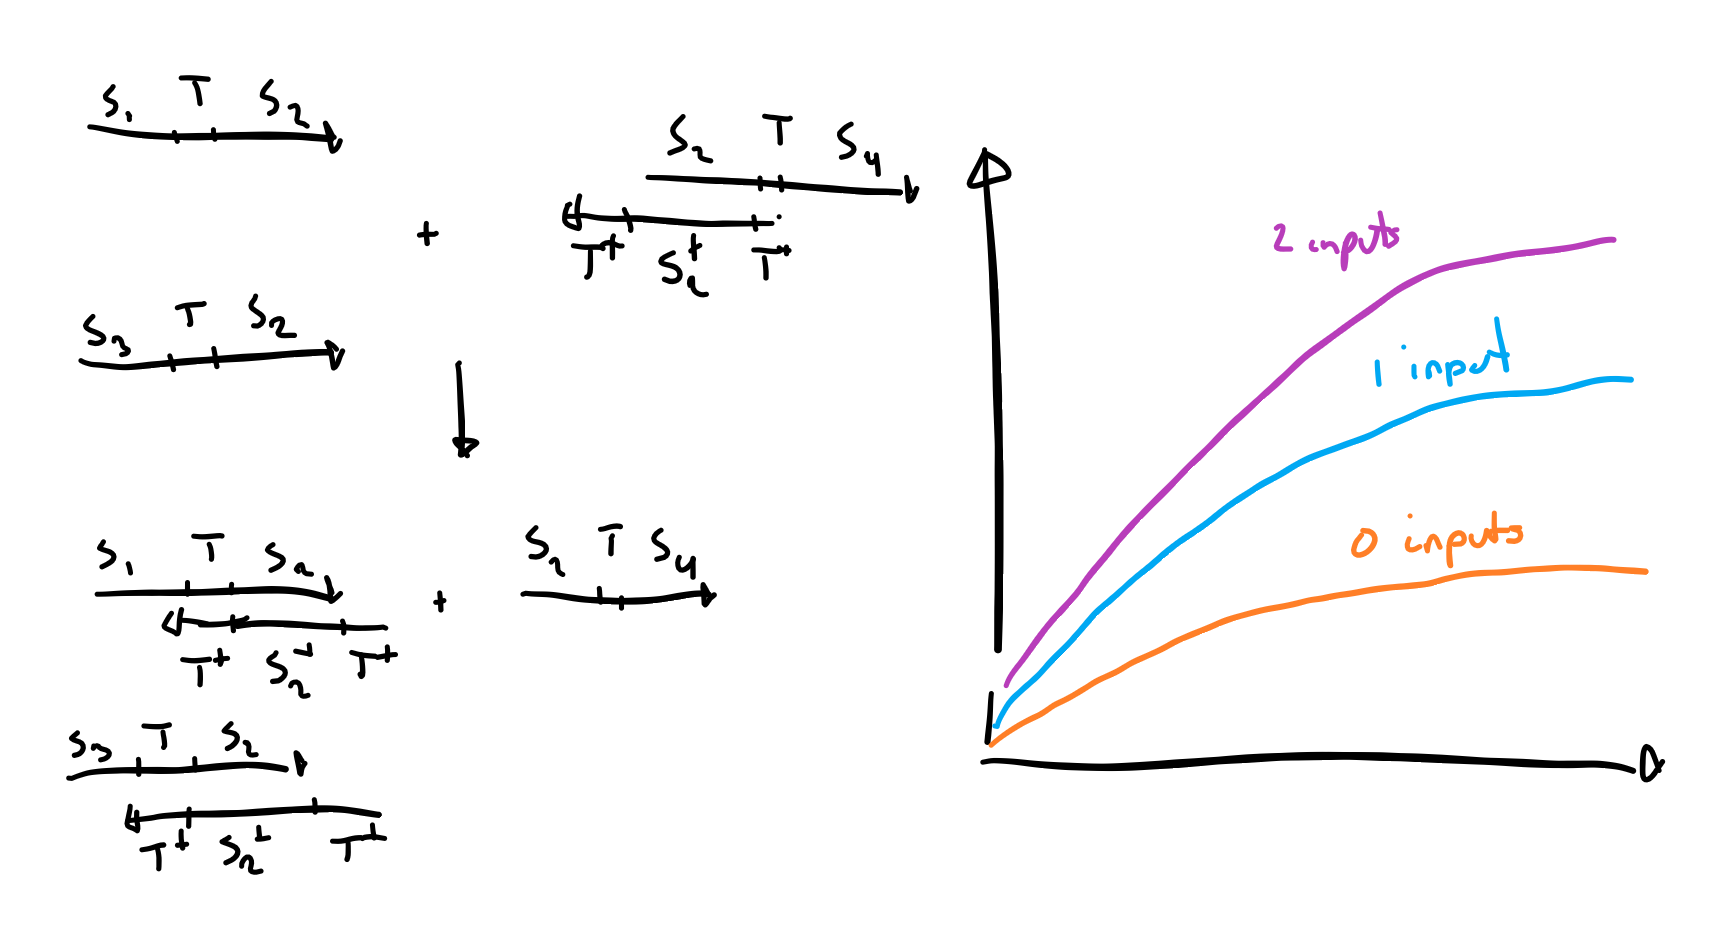
\includegraphics[width=\textwidth]{figures/seesaw_integration.tikz}
  \caption{}
  \label{seesaw_integration_reaction}
\end{subfigure}
\hfill
\begin{subfigure}[t]{.49\columnwidth}
  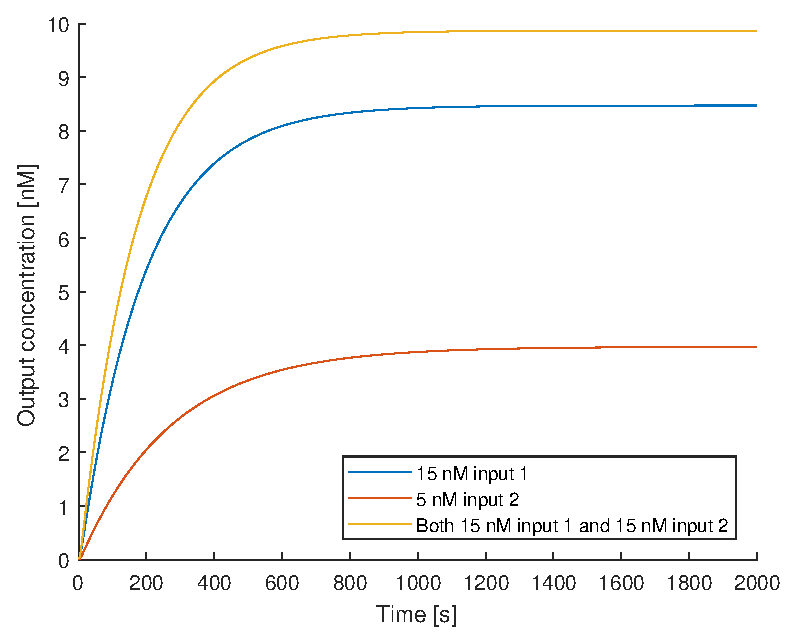
\includegraphics[width=\linewidth]{images/integration}
  \caption{}
  \label{seesaw_integration_time}
\end{subfigure}
\caption{\subref{seesaw_integration_reaction} Reaction of 2 input strands with an integration gate. The input strands have the same right recognition sequence $S_2$, and will both displace the top strand of the integration gate, releasing the output. \subref{seesaw_integration_time} Time analysis of the concentration of the output strand. The concentration of the integration gate is 20 nM. The first input of 15 nM increases the output strand concentration, compared to the second input of 5 nM. When both strands are added the concentration of output increases further.}
\label{seesaw_integration}
\end{figure}

\subsubsection{Weighting}
The inputs to the gate are weighted using their concentration. By making the integration gates concentration the sum of all the input concentrations, a high concentration of one input strand will contribute more to the activation than that of a low concentration, as shown in \fref{seesaw_integration_time}.

The weight is decided by the concentration of output of an input gate and its fuel strand (see \fref{seesaw_neuron}). The fuel serves the purpose of pushing the output of one gate to its target concentration, shown in \fref{seesaw_weighting}.

\begin{figure}[h]
\begin{subfigure}[t]{.49\textwidth}
  \includegraphics[width=\textwidth]{figures/seesaw_weighting.tikz}
  \caption{}
  \label{seesaw_weighting_reaction}
\end{subfigure}
\hfill
\begin{subfigure}[t]{.49\columnwidth}
  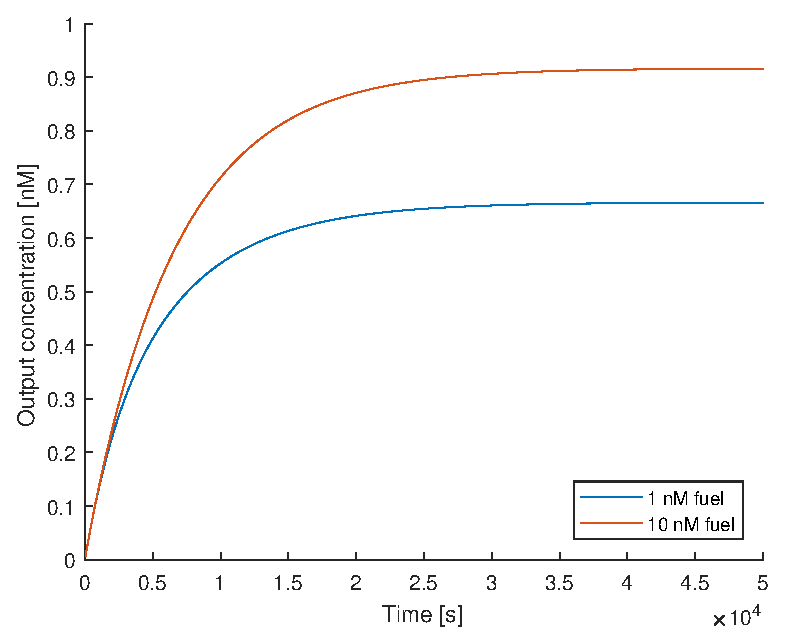
\includegraphics[width=\linewidth]{images/weighting}
  \caption{}
  \label{seesaw_weighting_analysis}
\end{subfigure}
\caption{\subref{seesaw_weighting_reaction} Reaction of an input strand with a gate and fuel. The input displaces the output strand from the gate, and the fuel blocks the reverse reaction, pushing the equilibrium towards the free output. \subref{seesaw_weighting_analysis} Time analysis of the concentration of the output strand. Input and gate concentration is initially 1 nM. When the fuel concentration is low (blue), the output concentration doesn't reach the initial gate concentration. When the fuel concentration is high (red), the output concentration is pushed closer towards its maximum concentration.}
\label{seesaw_weighting}
\end{figure}

A problem with this approach to weighting, is that the inputs can only contribute positively to the sum. In silico neural networks can use negative weights to simulate inhibitory synaptic connections, and is needed to implement many kind of boolean functions \cite{ZhaoYanling}. The in vitro network can't have negative concentrations of input sequences, so other approaches have to be considered. The problem can be solved using dual-rail logic \cite{Qian2011}, where each input is replaced by two inputs. The details of the dual-rail logic circuits is not a part of this project, and thus the networks will be limited to simple AND and OR circuits, since the NOT operation requires negative weights, and the XOR operation is not linearly separable \cite{ZhaoYanling}.

\subsubsection{Neuron}
By combining the discussed functional elements of the seesaw gate, a "neuron" can be created using strand displacement reactions, as depicted in \fref{seesaw_neuron}.

\begin{figure}[h]
\includegraphics[width=\textwidth]{figures/seesaw_neuron.tikz}
\caption{Schematic of a 2-input neuron implemented with seesaw gates. The neuron has an input gate for each input, which makes sure that the input concentration is higher than a given threshold before the input is registered. The gate and fuel concentrations in each input gate affects the weight of the input before it is sent to the integration gate. The integration gate collects the right recognition sequence from the input gates for the threshold gate. The threshold gate activates if the sum of the weighted inputs is larger than the threshold concentration of the treshold gate.}
\label{seesaw_neuron}
\end{figure}

Instead of displaying all strands of the seesaw circuit, each gate can be represented by a simplified schematic. The first input gate from \fref{seesaw_neuron} is shown in its simple version in \fref{seesaw_gate_simple}. Using the simple representation, the seesaw neuron from \fref{seesaw_neuron} can be simplified to the representation in \fref{seesaw_neuron_schematic}.

\begin{figure}[h]
  \begin{subfigure}[t]{.49\textwidth}
    \includegraphics[width=\textwidth]{figures/seesaw_gate.tikz}
    \caption{Seesaw gate strands}
  \end{subfigure}
  \quad
  \begin{subfigure}[t]{.49\textwidth}
    \includegraphics[width=\textwidth]{figures/seesaw_neuron_simple.tikz}
    \caption{Seesaw gate schematic}
  \end{subfigure}
  \caption{The strands and concentrations of the units of a seesaw gate can be represented to simplify larger diagrams.}
  \label{seesaw_gate_simple}
\end{figure}

\begin{figure}[h]
  \includegraphics[width=\textwidth]{figures/seesaw_neuron_schematic.tikz}
  \caption{The seesaw neuron from \fref{seesaw_neuron} shown as its simple representation.}
  \label{seesaw_neuron_schematic}
\end{figure}

The recommendations from the original paper \cite{Qian2011} is that each fuel strands concentrations is twice that of the gate concentration. The threshold concentration on the input gates (as shown in \fref{seesaw_neuron_schematic}) allows for concentrations of input strand less than 0.2 (relative concentration) to still be detected as 0.

The representation from \fref{seesaw_neuron_schematic} can further be simplified to the original perceptron shown in \fref{perceptron}. The seesaw neuron thus successfully implements all the required functionality of the artificial neuron, except for negative weights.

\subsubsection{Training}
The training algorithm typically used for digital perceptrons is based on the ability of the neurons to have negative weights and thresholds \cite{Gallant1990}. A modified algorithm is presented in the Qian et al 2011 \cite{Qian2011}, which works for dual rail circuits. For the circuits in this report without dual rail logic, the algorithm can be seen in \lref{codetraining}.

\begin{lstlisting}[float,floatplacement=h,caption=Pseudocode for the seesaw perceptron training algorithm, label=codetraining]
initialize all weights to 0 and threshold to 10
while training is incomplete
  for all the input sets
    find the output of the network from the input set
    if output is not correct
      mark training as incomplete
  if training is marked as incomplete
    increase the weights
\end{lstlisting}

The algorithm in \lref{codetraining} will keep increasing the weights until the output of the network matches the desired output. The input sets are taken from the truth table that the circuit should realize. If the circuit for example should realize the simple AND gate (see \tref{and_table}), the network is activated with the input rows from the truth table, and tested whether the output concentration equals (or is very close) to the output in the truth table.

\begin{table}[h]
\centering
\begin{tabular}{ccc}
  \hline
\multicolumn{1}{l}{\textbf{Input 1}} & \multicolumn{1}{l}{\textbf{Input 2}} & \multicolumn{1}{l}{\textbf{Output}} \\
\hline
0                                    & 0                                    & 0                                   \\
0                                    & 1                                    & 0                                   \\
1                                    & 0                                    & 0                                   \\
1                                    & 1                                    & 1 \\
\hline
\end{tabular}
\caption{Truth table for an AND gate.}
\label{and_table}
\end{table}

\subsection{Input translation}

As per design of the seesaw gate, the input sequences for the strand displacement neural network needs very specific left-recognition, right-recognition and toehold sequences. To detect sequences that does not have these elements, the sequences have to be translated. It has previously been demonstrated that miRNAs can be translated to other sequences \cite{Picuri2009}, by using two half-translators which are basic strand displacement reactions. An example of input translation can be seen in \fref{translator}.

\begin{figure}[h]
\includegraphics[width=\textwidth]{figures/translator.tikz}
\caption{Translation of arbitrary input sequences into the syntax required for the seesaw neural network. The input strand $ab$ displaces $bS_1T$ from the first half-translator. $bS_1T$ can then displace $S_1TS_2$ from the second half translator. This process successfully translates the input $ab$ into $S_1TS_2$, which can then be used for input in a neural network (see \fref{seesaw_neuron}).}
\label{translator}
\end{figure}

  \chapter{Method}
  % !TEX root = ../main.tex

% !TEX root = ../main.tex
\section{Perceptron simulation}

To simulate a perceptron with strand displacement reactions, the Visual DSD software was used to implement each of the subunits of a seesaw neuron discussed in the theory section. The syntax of the four subunits required to create a perceptron can be seen below (refer to the Visual DSD manual for the syntax \cite{dsdmanual}).

\begin{lstlisting}[label=dsd_subunits]
  def signal(N, S1L, S1, S1R, S2L, S2, S2R) = N * <S1L^ S1 S1R^ T^ S2L^ S2 S2R^>
  def threshold(N, S1R, S2L, S2, S2R) = N * {S1R^* T^*}[S2L^ S2 S2R^]
  def gate(N, S2L, S2, S2R, S3L, S3, S3R) = N * {T^*}[S2L^ S2 S2R^ T^]<S3L^ S3 S3R^>
  def fuel(N, S1L, S1, S1R) = N * <S1L^ S1 S1R^ T^ Sf>
\end{lstlisting}

Each of the subunits can be called with the desired left and right recognition sequences, when combining them for larger units. Note that each of the recognition sequences (S1 for example) is split into 3 (S1L, S1, S1R). This is needed to implement the threshold gate, which has a short part of the left recognition sequence (\fref{seesaw_thresholding}).


The actual perceptron can be pieced together by combining the subunits from \lref{dsd_subunits}. The 2-input AND using seesaw gates seen in \fref{seesaw_gate}, can be written in Visual DSD as:

\begin{lstlisting}[label=dsd_and_gate]
  (
  (* First input gate *)
  signal(0.9, S1L, S1, S1R, S2L, S2, S2R) |
  threshold(0.2, S1R, S2L, S2, S2R) |
  gate(1.0, S2L, S2, S2R, S3L, S3, S3R) |
  fuel(2, S2L, S2, S2R) |
  (* Second input gate*)
  signal(0.9, S4L, S4, S4R, S5L, S5, S5R) |
  threshold(0.2, S4R, S5L, S5, S5R) |
  gate(1.0, S5L, S5, S5R, S3L, S3, S3R) |
  fuel(2, S5L, S5, S5R) |
  (* Summation gate *)
  gate(2, S3L, S3, S3R, S6L, S6, S6R) |
  (* Thresholding gate *)
  threshold(1.5, S3R, S6L, S6, S6R) |
  gate(1.0, S6L, S6, S6R, S7L, S7, S7R) |
  fuel(2, S6L, S6, S6R)
  )
\end{lstlisting}

To abstract from the Visual DSD syntax, a transpiler was created in Javascript which can generate the needed Visual DSD code for perceptrons of variable input size. The transpiler can take a truth table defined as an array, and generates the needed Visual DSD code to create a perceptron of required input size.

To train the perceptron, the initial idea was to simply train a software perceptron to a given truth table, and use the found weights and thresholds in the seesaw perceptron. This idea proved too naive, as the weights and thresholds from a software perceptron did not produce the same outputs in a seesaw perceptron. The solution was to generate the Visual DSD code, run it through the command-line version of the Visual DSD software, and simulate the output concentration of the perceptron. This output could then be compared to the expected output from the truthtable, and the weights adjusted using the algorithm discussed in the theory section.

It was not possible to create a web application with a user friendly interface for designing the perceptron, as was done with the software training \cite{neuralcircuit}. The command-line version of the Visual DSD software preferably needs to be run on a Windows machine, for which no free hosting could be found in time. The code is still available on Github for running locally on Windows machines \cite{neuralcompiler}.

% !TEX root = ../main.tex
\section{Translation}

\subsection{Design}

The translator was designed to output the sequence CUAGACUGAAGCUCCUUGAGG, which is the sequence that can activate a FRET tile previously designed in the group [SOURCE AND FIND OUT WHICH MIRNA FROM WHERE]. The input was not specifically chosen, but generated by Nupack to fulfill the design parameters. Two versions of the translator were designed, one where the translator subunits annealed with 10 bp (\lref{codeshort}), and one where they annealed with 20 bp (\lref{codelong}). The long translator was closer to the setup of the original DNA translator \cite{Picuri2009}, which had annealing lengths of 23-25 bp.

When transcribing the RNA using the T7 RNA polymerase, the sequences are going to start with GG [SOURCE], so these were included in the design. Repeats of identical nucleotides were also prevented [REASON]. The result of the Nupack designed RNA sequences can be seen in \tref{rna} (refer to \fref{translator_short_subunits} and \fref{translator_long_subunits} for strand names).

\begin{figure}[h]
\centering
\includegraphics[width=\textwidth]{figures/translator_short_naming.tikz}
\caption{Sequence naming of the short translator sequences (see table \ref{rna_strands}).}
\label{translator_short_subunits}
\end{figure}

\begin{figure}[h]
\centering
\includegraphics[width=\textwidth]{figures/translator_long_naming.tikz}
\caption{Sequence naming of the long translator sequences (see table \ref{rna_strands}).}
\label{translator_long_subunits}
\end{figure}

To transcribe the RNA sequences, the RNA was converted to DNA, and the T7 promoter was added to the strands. The reverse complement of the strands was found, to serve as the template strand. The T7 RNA polymerase does not need the full template to be double-stranded, only the promoter sequence [SOURCE], so the resulting template will be the DNA version of the reverse complement of the target RNA (plus the reverse complement of the promoter), annealed with the promoter sequence (depicted in \fref{rna_to_dna_process}). A program was written to convert the target RNA sequences to their DNA template directly on the output from Nupack, and format it for batch IDT ordering \cite{nupackorder}.

\begin{figure}[h]
\centering
\includegraphics[width=\textwidth]{figures/rna_to_dna.tikz}
\caption{DNA template from RNA sequence for the T7 RNA polymerase.}
\label{rna_to_dna_process}
\end{figure}

\subsection{Transcription}

\begin{table}
\begin{adjustbox}{width=\columnwidth}
\begin{tabular}{llll}
\hline
\textbf{Name}      & \textbf{Short} & \textbf{Sequence}                                           & \textbf{Length} \\
\hline
T7 promoter        & 0          & GGTAATACGACTCACTATAG                                           & 20     \\
Short 1            & 1          & CCTCAAGGAGCTTCAGTCTAGCCCTATAGTGAGTCGTATTACC                    & 43     \\
Short 2            & 2          & CTCCTTGAGGCACATAACTCCCCTATAGTGAGTCGTATTACC                     & 42     \\
Short 3            & 3          & CACATAACTCTACTAAATCTCCCTATAGTGAGTCGTATTACC                     & 42     \\
Short 4            & 4          & GAGTTATGTGCCTCAAGGAGCCCTATAGTGAGTCGTATTACC                    & 42     \\
Short 5            & 5          & AGATTTAGTAGAGTTATGTGCCCTATAGTGAGTCGTATTACC                     & 42     \\
Long 1             & 6          & GTCAATTCGCCTCAAGGAGCTTCAGTCTAGCCCTATAGTGAGTCGTATTACC           & 52     \\
Long 2             & 7          & GCTCCTTGAGGCGAATTGACCCATCTTCATTCTACTCCTACCCTATAGTGAGTCGTATTACC & 62     \\
Long 3             & 8          & CCATCTTCATTCTACTCCTATACCTCAATCCCCTATAGTGAGTCGTATTACC           & 52     \\
Long 4             & 9          & TAGGAGTAGAATGAAGATGGGTCAATTCGCCTCAAGGAGCCCCTATAGTGAGTCGTATTACC & 62     \\
Long 5             & 10         & GATTGAGGTATAGGAGTAGAATGAAGATGGCCCTATAGTGAGTCGTATTACC           & 52     \\
Beacon fluorophore & 11         & CGGCTAGACTGAA                                                  & 13     \\
Beacon quencher    & 12         & CCTCAAGGAGCTTCAGTCTAGCCG                                       & 24 \\
\hline
\end{tabular}
\end{adjustbox}
\caption{Sequences and names of the DNA strands used for transcription.}
\label{dna_strands}
\end{table}

\begin{table}
\begin{adjustbox}{width=\columnwidth}
\begin{tabular}{llll}
\hline
\textbf{Name}      & \textbf{Short} & \textbf{Sequence}                                           & \textbf{Length} \\
\hline
Short 1            & 1          & GGCUAGACUGAAGCUCCUUGAGG                    & 23     \\
Short 2            & 2          & GGGAGUUAUGUGCCUCAAGGAG                     & 22     \\
Short 3            & 3          & GGAGAUUUAGUAGAGUUAUGUG                     & 22     \\
Short 4            & 4          & GGCUCCUUGAGGCACAUAACUC                     & 22     \\
Short 5            & 5          & GGCACAUAACUCUACUAAAUCU                     & 22     \\
Long 1             & 6          & GGCUAGACUGAAGCUCCUUGAGGCGAAUUGAC           & 32     \\
Long 2             & 7          & GGUAGGAGUAGAAUGAAGAUGGGUCAAUUCGCCUCAAGGAGC & 42     \\
Long 3             & 8          & GGGAUUGAGGUAUAGGAGUAGAAUGAAGAUGG           & 32     \\
Long 4             & 9          & GGGCUCCUUGAGGCGAAUUGACCCAUCUUCAUUCUACUCCUA & 42     \\
Long 5             & 10         & GGCCAUCUUCAUUCUACUCCUAUACCUCAAUC           & 32     \\
% Beacon fluorophore & 11         & CGGCTAGACTGAA                                                  & 13     \\
% Beacon quencher    & 12         & CCTCAAGGAGCTTCAGTCTAGCCG                                       & 24 \\
\hline
\end{tabular}
\end{adjustbox}
\caption{Sequences and names of the transcribed RNA strands.}
\label{rna_strands}
\end{table}

The oligos from IDT was dissolved in TE buffer (\tref{te_buffer}) to an approximate concentration of 120 \si{\micro}M, based on the quantity of substance written on the tubes. The final concentration desired was 100 \si{\micro}M, but due to a risk of inaccurate substance quantities, the dissolved concentration was chosen to be slightly above. The oligos could then be further diluted after measuring their absorbance on the Nanodrop.

After dissolving the oligos, the absorbance of each sample was measured on the Nanodrop in triplets. A program was written which can take the .csv output of the Nanodrop, and calculate the concentration based on each strands extinction coefficient \cite{nanodropimport}.

The measured concentrations (\fref{oligo_concentrations}) was used to dilute the samples further, to a concentration of 100 \si{\micro}M.

To anneal the templates to the promoter, each of the template strands was mixed with equal amounts of promoter strand in annealing buffer (\tref{annealing_buffer}), to a final concentration of 1 \si{\micro}M. The mixed samples were then heated to 90$^\circ$ C for 5 minutes, and left to cool down to room temperature.

To check if samples annealed properly, they were run on a 20\% native PAGE gel for 3 hours. Each lane was loaded with 50 \si{\micro}l sample, and 10 \si{\micro}l native loading buffer (\tref{native_buffer}). Afterwards the gel was stained in SYBR Gold, and visualised on the Typhoon scanner. The result of the scan can be seen in figure \ref{fig:promoter_annealing_gel}.

\begin{figure}
\centering
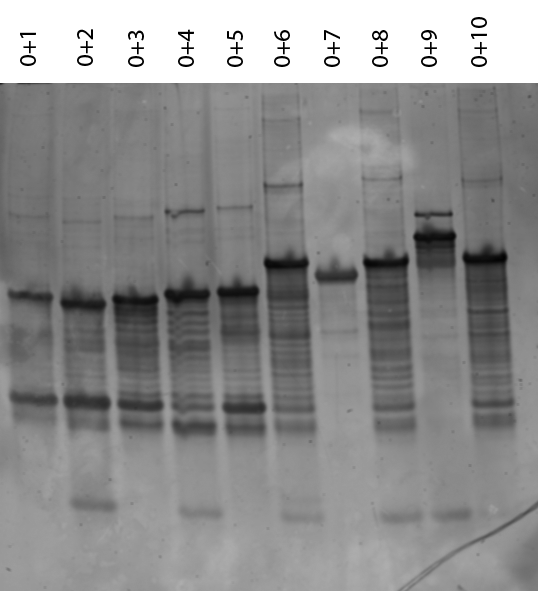
\includegraphics[width=\columnwidth]{images/promoter_annealing_gel.png}
\caption{Typhoon scan of SYBR Gold stained native PAGE gel, with the annealed templates and promoter strands. The lanes are labelled by which strands are annealed (see table \ref{dna_strands}).}
\label{fig:promoter_annealing_gel}
\end{figure}

As can be seen in figure \ref{fig:promoter_annealing_gel}, the darkest bands is the annealed samples. The samples for the short translator runs as about the same size, while there is bigger variation in the long translator samples, as expected based on table \ref{dna_strands}. The exact positions of the long translator samples does not match with the sequence length, though this can be explained by secondary structures of the single-stranded part of the sample. The shorter bands visible below, is probably excess promoter, other secondary structures, and shorter sequences from synthesis errors. No lane with ladder was run, so the exact position of the bands can't be commented on.

To get the desired RNA sequences, a transcription reaction was run with each of the annealed DNA templates, according to table \ref{transcription1}.

\begin{table}\centering
\begin{tabular}{llll}
  \hline
                       & \textbf{Initial conc.} & \textbf{Final conc.} & \textbf{Volume} \\ \hline
  Transcription buffer & 10X                    & 1X                   & 10 \si{\micro}L           \\
  DTT                  & 100 mM                 & 10 mM                & 10 \si{\micro}L           \\
  NTP mix              & 25 mM                  & 2.5 mM               & 10 \si{\micro}L           \\
  Template             & 500 nM                 & 50 nM                & 10 \si{\micro}L           \\
  T7 RNA polymerase    &                        &                      & 1 \si{\micro}L            \\
  Nuclease-free water  &                        &                      & 59 \si{\micro}L           \\
  Total                &                        &                      & 100 \si{\micro}L          \\ \hline
\end{tabular}
\caption{Mixing of compounds for the first transcription done on the templates for both the short and long translater.}
\label{transcription1}
\end{table}

The samples were left overnight at 37$^\circ$ C. The day after, 1 \si{\micro}L of RNAse free DNAse was added to the samples, and heated for 37$^\circ$ C for an hour. Afterwards, 100 \si{\micro}L of denaturing loading buffer was added to each sample, and 10 ul of the DNA 0 and DNA 5 strands was mixed with 10 \si{\micro}L of denaturing loading buffer, and heated for 5 minutes at 90$^\circ$ C.

To purify the RNA, the transcribed sequences and controls were run on a 20\% denaturing PAGE gel, for 4 hours at 20 W.

The RNA product should be visible in UV shadowing, but no product was seen. The gel was then stained with SYBR Gold and scanned on the Typhoon. The result can be seen in figure \ref{transcription_1}.

\begin{figure}
  \begin{subfigure}{0.49\textwidth}
  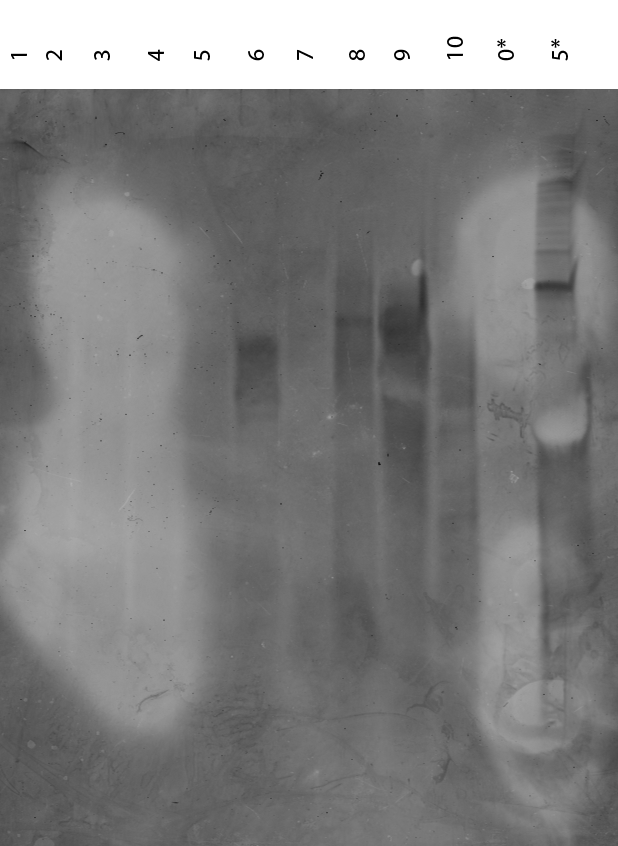
\includegraphics[width=\textwidth]{images/translator_transcription_1.png}
  \caption{Typhoon scan of SYBR Gold stained native PAGE gel, with the transcribed RNA strands in lanes 1-10, and controls in 11 and 12. The lanes are labelled by which strands are annealed (see \tref{rna_strands}). The asterix refers to the DNA strands in \tref{dna_strands}.}
  \label{transcription_1}
  \end{subfigure}
  \begin{subfigure}{0.49\textwidth}
    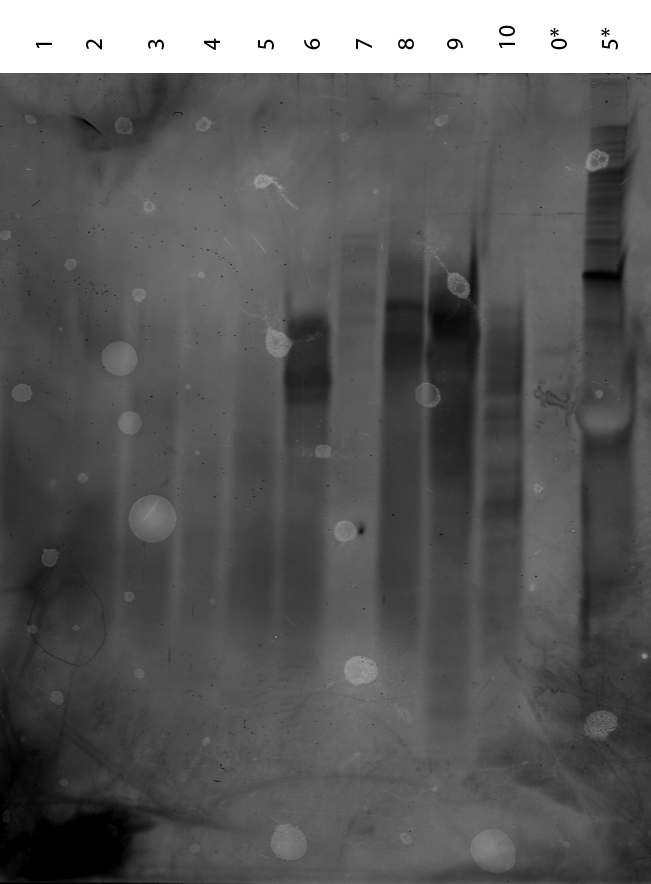
\includegraphics[width=\textwidth]{images/translator_transcription_2.png}
    \caption{Typhoon scan of SYBR Gold stained native PAGE gel, with the transcribed RNA strands in lanes 1-10, and controls in 11 and 12. The lanes are labelled by which strands are annealed (see table \ref{rna_strands}). The asterix refers to the DNA strands in table \ref{dna_strands}.}
    \label{transcription_2}
  \end{subfigure}
\end{figure}

As can be seen in \fref{transcription_1}, the gel wasn't stained long enough, so after restaining it in SYBR Gold, it was scanned again.

The lanes 1-10 in \fref{transcription_2} does not show distinct bands. There seems to be more product from the long translator transcriptions (lanes 6-10), than in the short ones (lanes 1-5). Even the controls which were loaded in equal amounts does not show up in equal strength. Since the gel from the DNA annealing was run without any controls, it was difficult to see if there was any errors in the annealing. Another 20\% native PAGE gel was run with the annealed DNA, using the single stranded oligos as control. To simplify the experiment while trying to find the error, only the short translator sequences were used.

\begin{figure}[H]
\centering
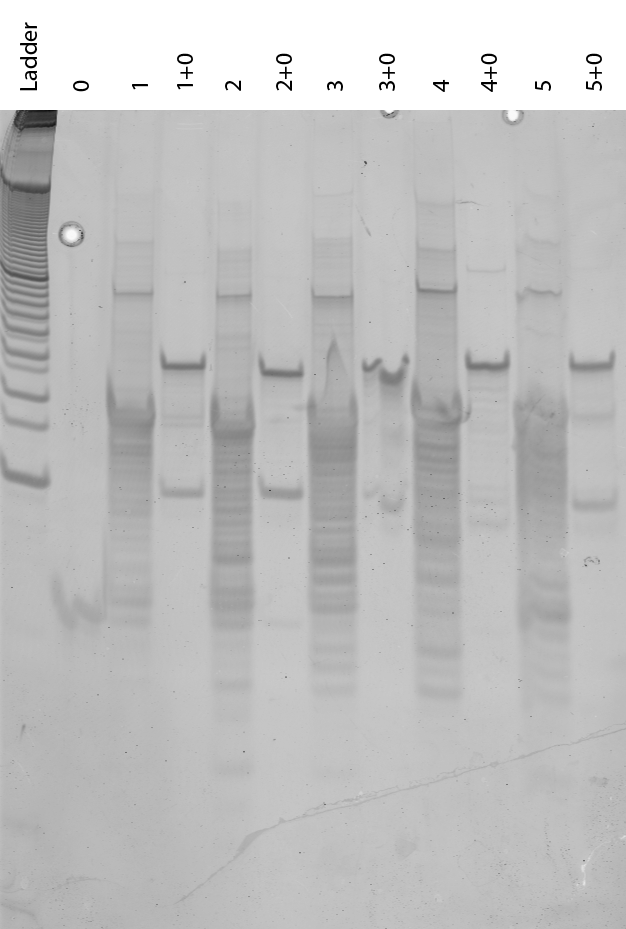
\includegraphics[width=200pt]{images/translator_annealing_2.png}
\caption{The annealed oligos together with controls and a 10 nt ladder. The lanes are labelled with the oligo names given in \tref{dna_strands}. The plus symbol denotes which strands are annealed.}
\label{translator_annealing_2}
\end{figure}

The results of \fref{translator_annealing_2} still shows that the templates have annealed with the promoter, and runs as about 40-50 bp. The expected size is around 60 bp (sum of promoter and template), but it is difficult to say how a partly annealed structure will run on a native gel. The new gel does however show that the bands in the annealed lanes below the assumed product, might not be excess promoter. The promoter is seen in the second lane, and lies below the bands in the annealed structure thought to be excess promoter. The bands below the product might be due to secondary structures of each of the template strands, but comparing with \fref{short_secondary_structures}, the band in the 5+0 lane would be expected to be less visible, as strand 5 has no secondary structure.

Despite the unexplained bands from the annealing, a new transcription was run on the short template strands to see if better results could be obtained. The transcription was done using the previous protocol, and run on a gel. The UV shadowing still did not show any visible product, so the gel was scanned to check for bands.

\begin{figure}[H]
\centering
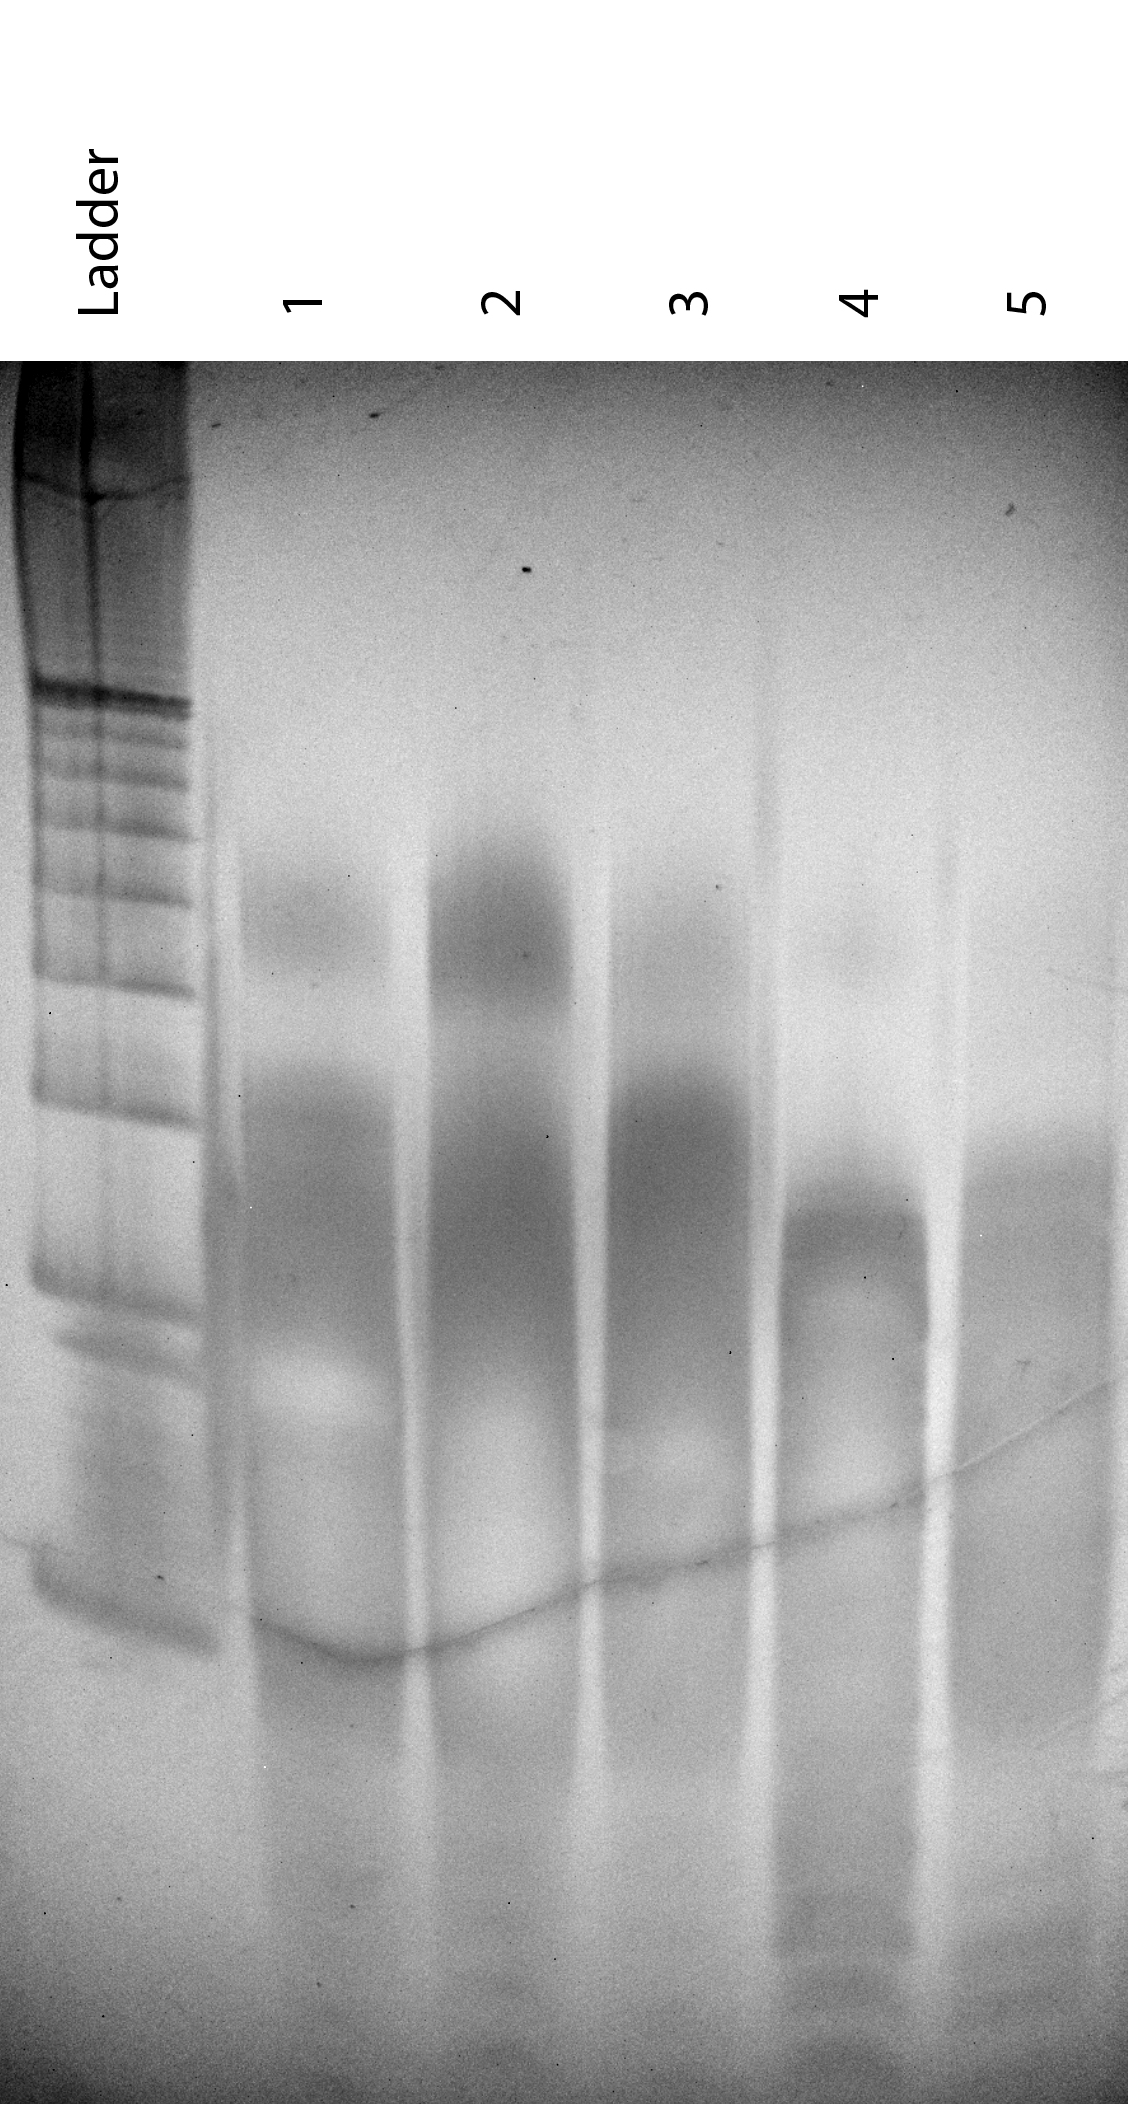
\includegraphics[width=150pt]{images/translator_transcription_3.png}
\caption{The transcribed short translator sequences and a 10 nt ladder. The lanes are labelled with the oligo names given in \tref{rna_strands}.}
\label{translator_transcription_3}
\end{figure}

As seen in \fref{translator_transcription_3}, still no clear bands with RNA product was visible. After checking all buffers and materials, it was learned that the T7 polymerase that was used was from 2013, and might have been too old to still function properly. A fresh T7 polymerase was used for a new transcription, same as the previous protocol. The UV shadowing did show some distinct bands this time, so the bands was cut out for purification. The purification was done using the precipitation protocol \cite{precipitationprotocol}. After purification the pellets were dissolved in 100 \si{\micro}L TE buffer, their absorbance measured on the Nanodrop, and their concentration calculated using their extinction coefficients.

To check that the purification worked, 2 \si{\micro}L of each sample with 1 \si{\micro}L of denaturing loading buffer was run on a 20\% denaturing gel, stained with SYBR Gold, and visualised on the Typhoon.

\begin{figure}[H]
\centering
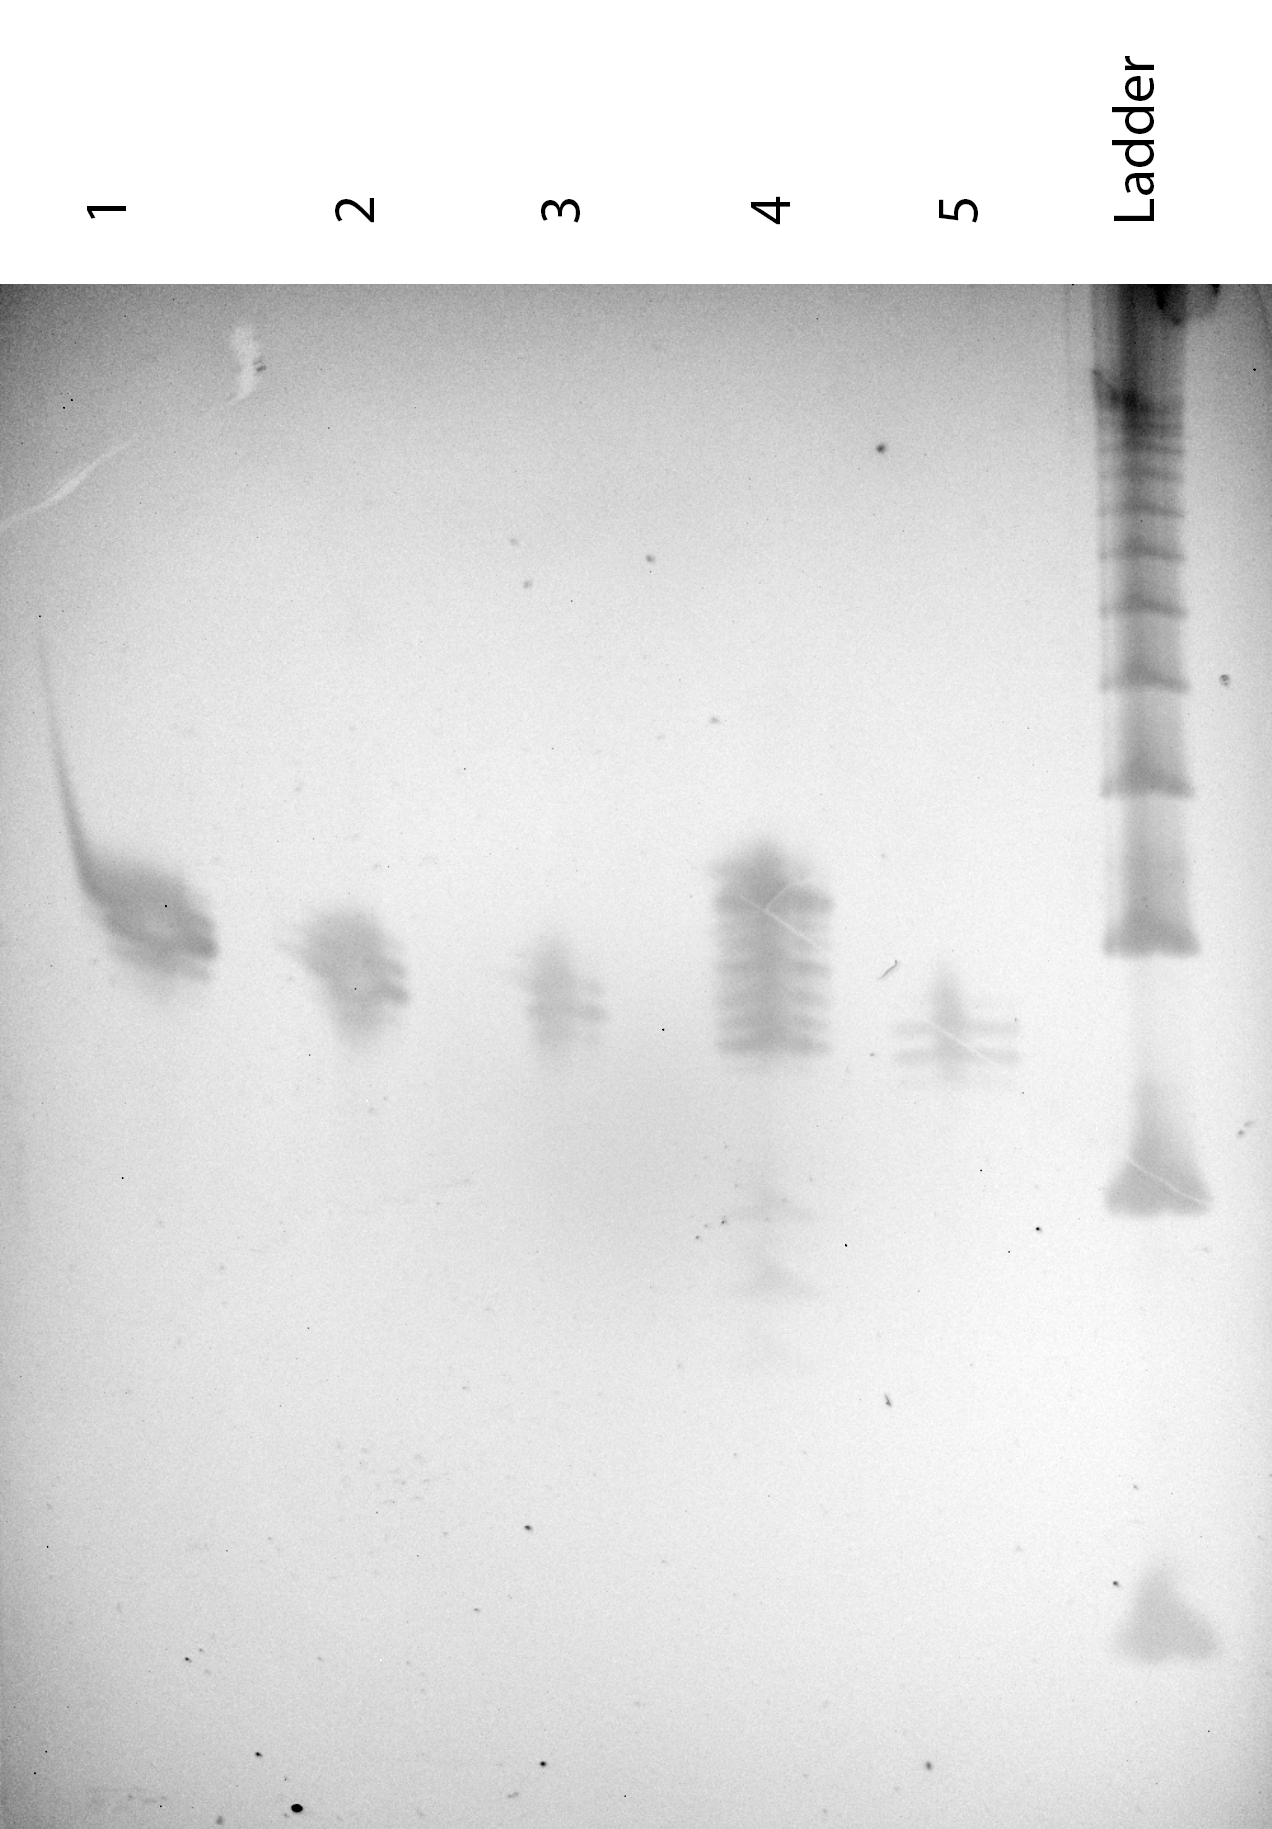
\includegraphics[width=150pt]{images/translator_transcription_purified.png}
\caption{The purified short translator RNA oligos.}
\label{translator_transcription_purified}
\end{figure}

\fref{translator_transcription_purified} shows that the RNA has been isolated, but is not very pure. It is possible that when cutting out the RNA from the gel before purification, too large an area was taken. The target RNA sequences were still expected to be in the purified samples (albeit not very pure), and it has previously been shown that strand displacement reactions can work with unpurified components \cite{Thubagere2017}, so the experiment continued with the current RNA.

Based on the concentrations in \fref{translator_transcription_concentration}, the samples were further diluted in RNAse-free water to 2 \si{\micro}M for the translator strands (1-4) and 1 \si{\micro}M for the input strand (5). Then 25 \si{\micro}L of each of the translator strands were mixed with their respective counterpart (1+2 and 3+4) to a final concentration of 1 \si{\micro}M in 50 \si{\micro}L.

At this point, the reporter samples were also mixed and diluted in RNAse-free water to the same concentration as the translator subunits. To each of the subunits and the reporter, 5 \si{\micro}L of 10X annealing buffer was added. The samples were heated at 90$^\circ$ C for 5 minutes, and cooled off at room temperature.

To check if the subunits and reporter annealed properly, they were run on a 20\% native PAGE gel with the single strands as control. It was expected that the fluorophore would be visible at the same wavelength as SYBR Gold, so a scan without staining should show the free fluorophore (and not the quenched fluorophore in the annealed reporter).

\begin{figure}
\begin{subfigure}{.49\columnwidth}
  \centering
  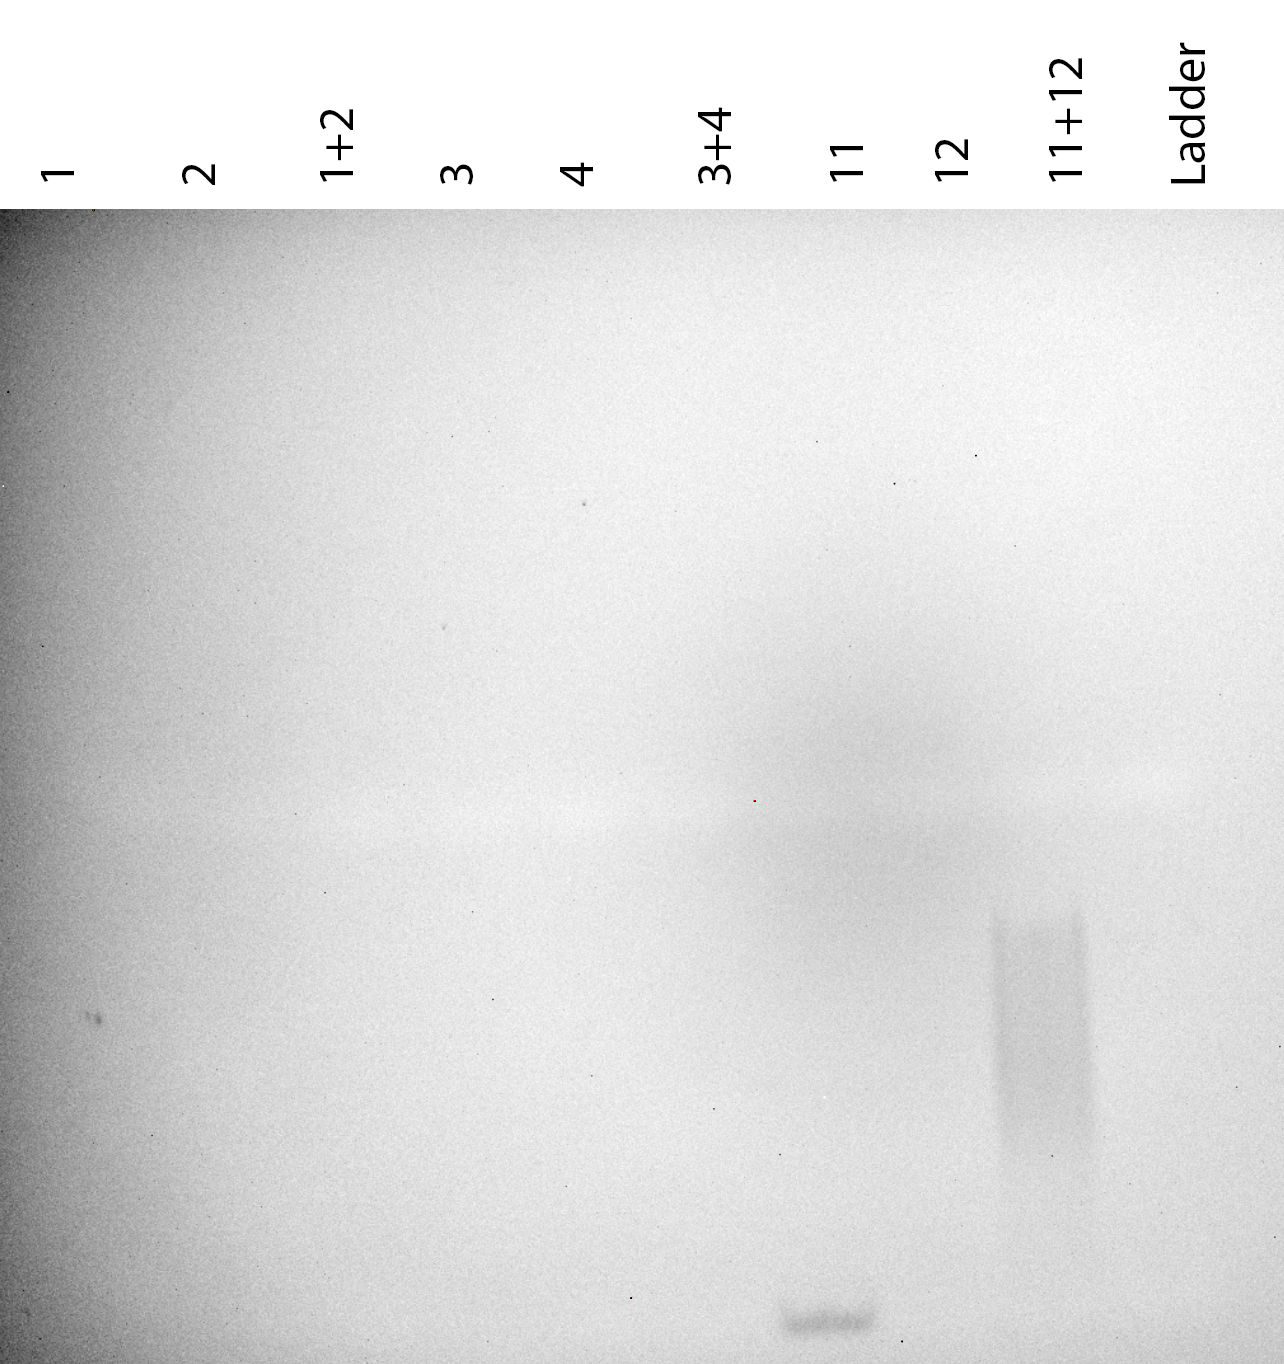
\includegraphics[width=\linewidth]{images/transcription_annealed_nostain.png}
  \caption{Not stained}
\end{subfigure}
\hfill
\begin{subfigure}{.49\columnwidth}
  \centering
  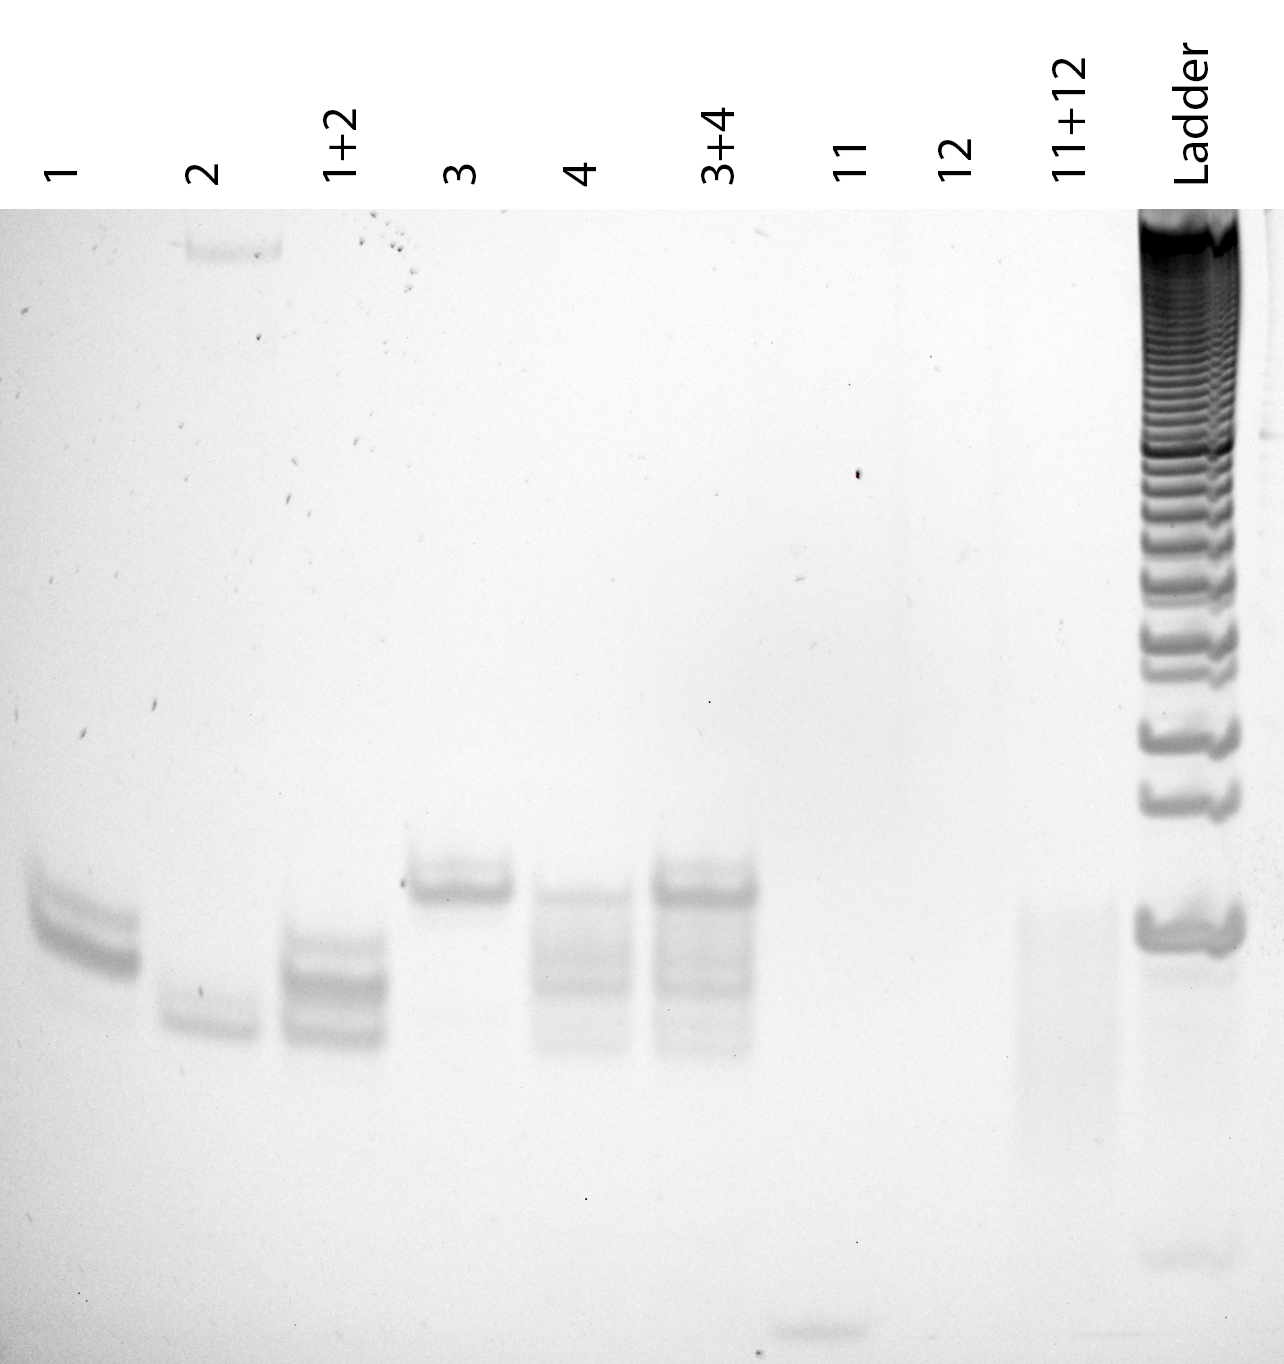
\includegraphics[width=\linewidth]{images/transcription_annealed_stain.png}
  \caption{Stained}
\end{subfigure}
\caption{The annealed short translator subunits and reporter, with the single strands as controls, and a 10 nt ladder.}
\label{transcription_annealed}
\end{figure}

As seen in \fref{transcription_annealed}, the fluorophore clearly shows up in the unstained scan, and gets partly quenched and moves up when annealed to its quencher. The smear in the annealed reporter might be due to synthesis errors in the quencher strand.

In the stained scan, the annealed translator subunits does not seem to have annealed at all. Comparing with the controls, the strands that was supposed to have annealed, merely looks like the sum of the single strands. There is a few reasons why this could have happened. The RNA that was purified from gel was not the correct sequences, the annealing was not carried out correctly, or the strands simply doesn't anneal very good.

To check the strength of the annealing, the strands were analyzed in Nupack. The result (\fref{annealing_concentration}) shows that the short translator sequences does not anneal as good as the long ones.

\begin{figure}
\begin{subfigure}[b]{.49\columnwidth}
  \centering
  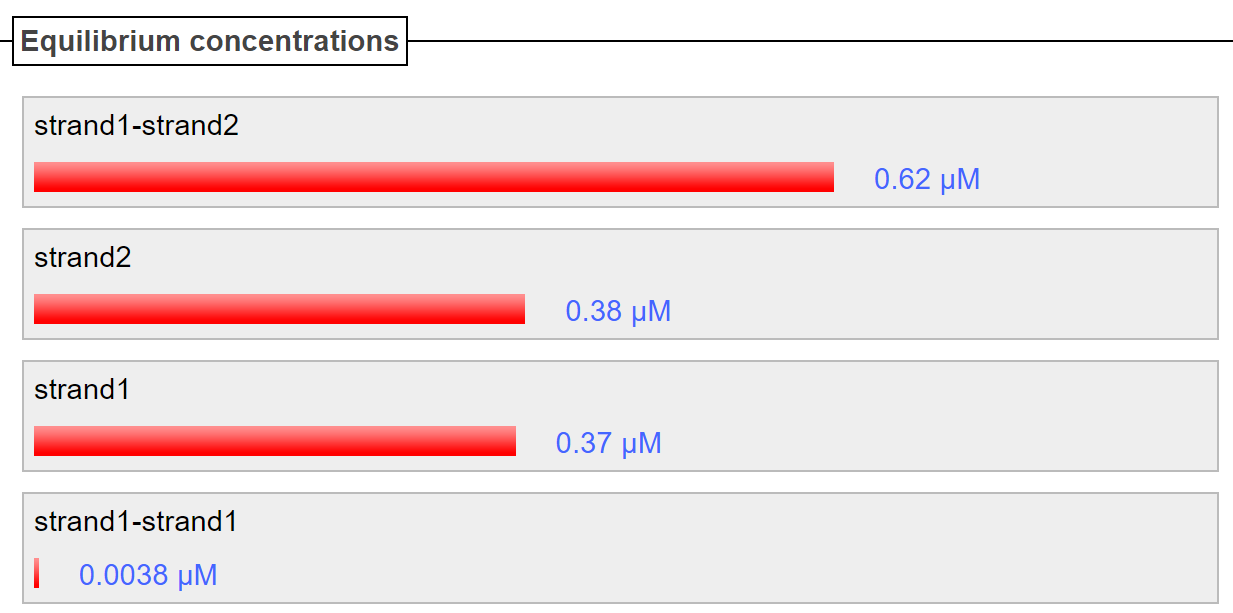
\includegraphics[width=\linewidth]{images/short_annealing_concentration.png}
  \caption{Equilibrium concentration of the short translator strands 1 and 2.}
\end{subfigure}
\hfill
\begin{subfigure}[b]{.49\columnwidth}
  \centering
  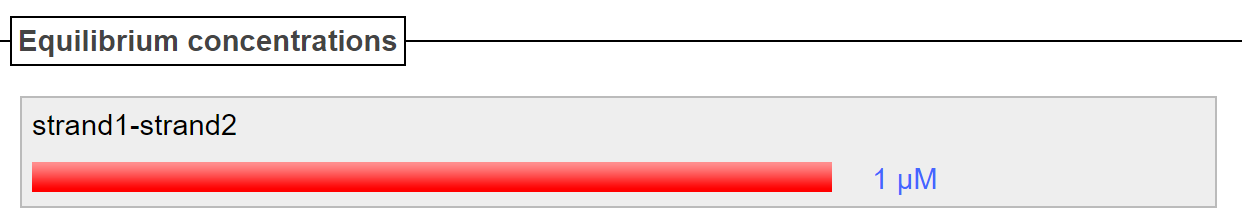
\includegraphics[width=\linewidth]{images/long_annealing_concentration.png}
  \caption{Equilibrium concentration of the long translator strands 6 and 7.}
\end{subfigure}
\caption{Nupack analysis of the equilibrium concentrations of the first subunit of the short and long translator.}
\label{annealing_concentration}
\end{figure}

Due to time constraints, the focus moved towards the long translator sequences, as they were expected to provide better results.

A new transcription for the long translator sequences was prepared using the previous protocol. The transcription was run for 3 hours at 37$^\circ$ C and then run on a 20\% denaturing PAGE gel for 2 hours. No immediate product was visible, but a scan revealed that some RNA had been produced.

\begin{figure}
\centering
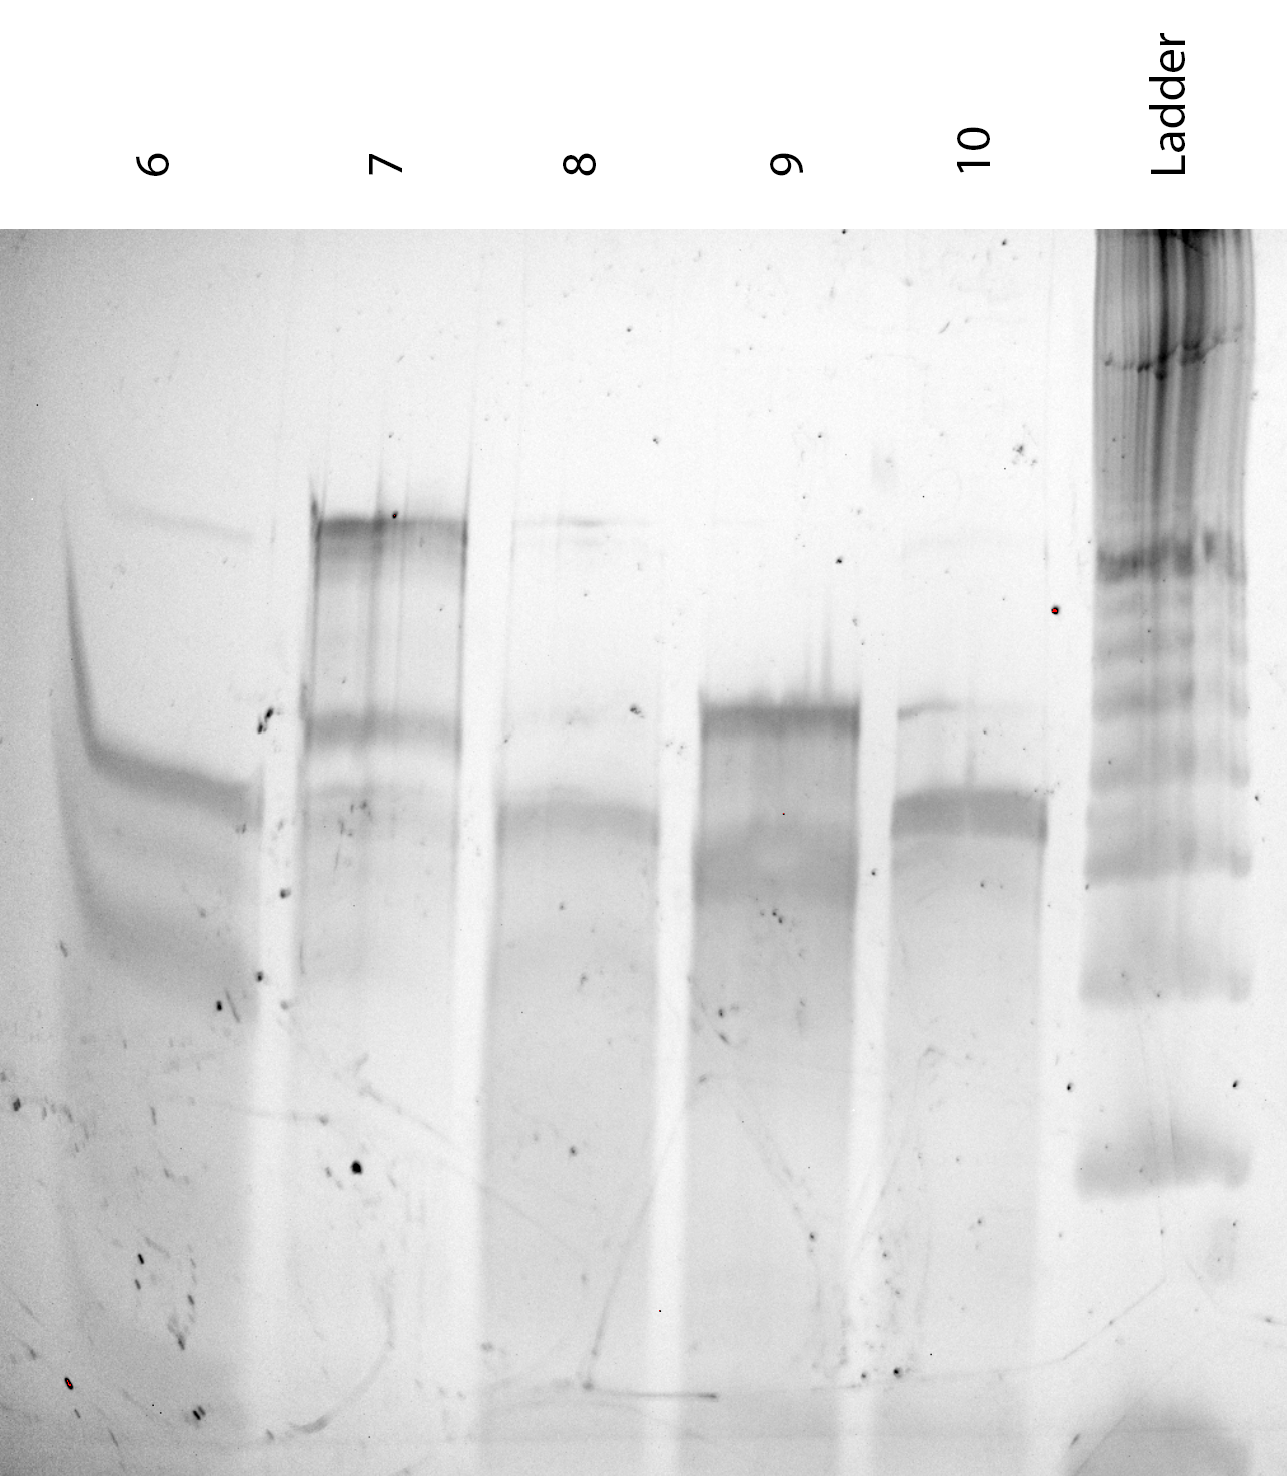
\includegraphics[width=150pt]{images/translator_transcription_long_1.png}
\caption{Transcription of the long translator sequences with a 10 nt ladder.}
\label{translator_transcription_long_1}
\end{figure}

As seen in \fref{translator_transcription_long_1}, some RNA was produced so the concentration of nucleotides in the reaction was increased to get enough RNA to be visible in UV shadowing. The transcription protocol was also changed to one recommended from the supplier of the T7 polymerase \cite{nebtranscription}, to ensure that the polymerase was not the problem (\tref{transcription2}). The new transcription was carried out as the previous one, and revealed a single band (strand 9) in UV shadowing, but the rest of the templates had not produced enough RNA to be purified. A scan revealed once again that RNA had been produced, but the right product could not be isolated.

\begin{table}\centering
\begin{tabular}{llll}
  \hline
   & \textbf{Initial conc.} & \textbf{Final conc.} & \textbf{Volume} \\ \hline
  Transcription buffer & 10X                    & 1X                   & 4 \si{\micro}L           \\
  DTT                  & 100 mM                 & 5 mM                & 2 \si{\micro}L           \\
  NTP mix              & 25 mM                  & 2.5 mM               & 4 \si{\micro}L           \\
  Template             & 500 nM                 & 250 nM                & 20 \si{\micro}L           \\
  T7 RNA polymerase    &                        &                      & 4 \si{\micro}L            \\
  Nuclease-free water  &                        &                      & 6 \si{\micro}L           \\
  Total                &                        &                      & 40 \si{\micro}L          \\ \hline
\end{tabular}
\caption{Mixing of compounds based on the transcription protocol from NEB, for the second transcription of the long translator.}
\label{transcription2}
\end{table}

\begin{figure}
\centering
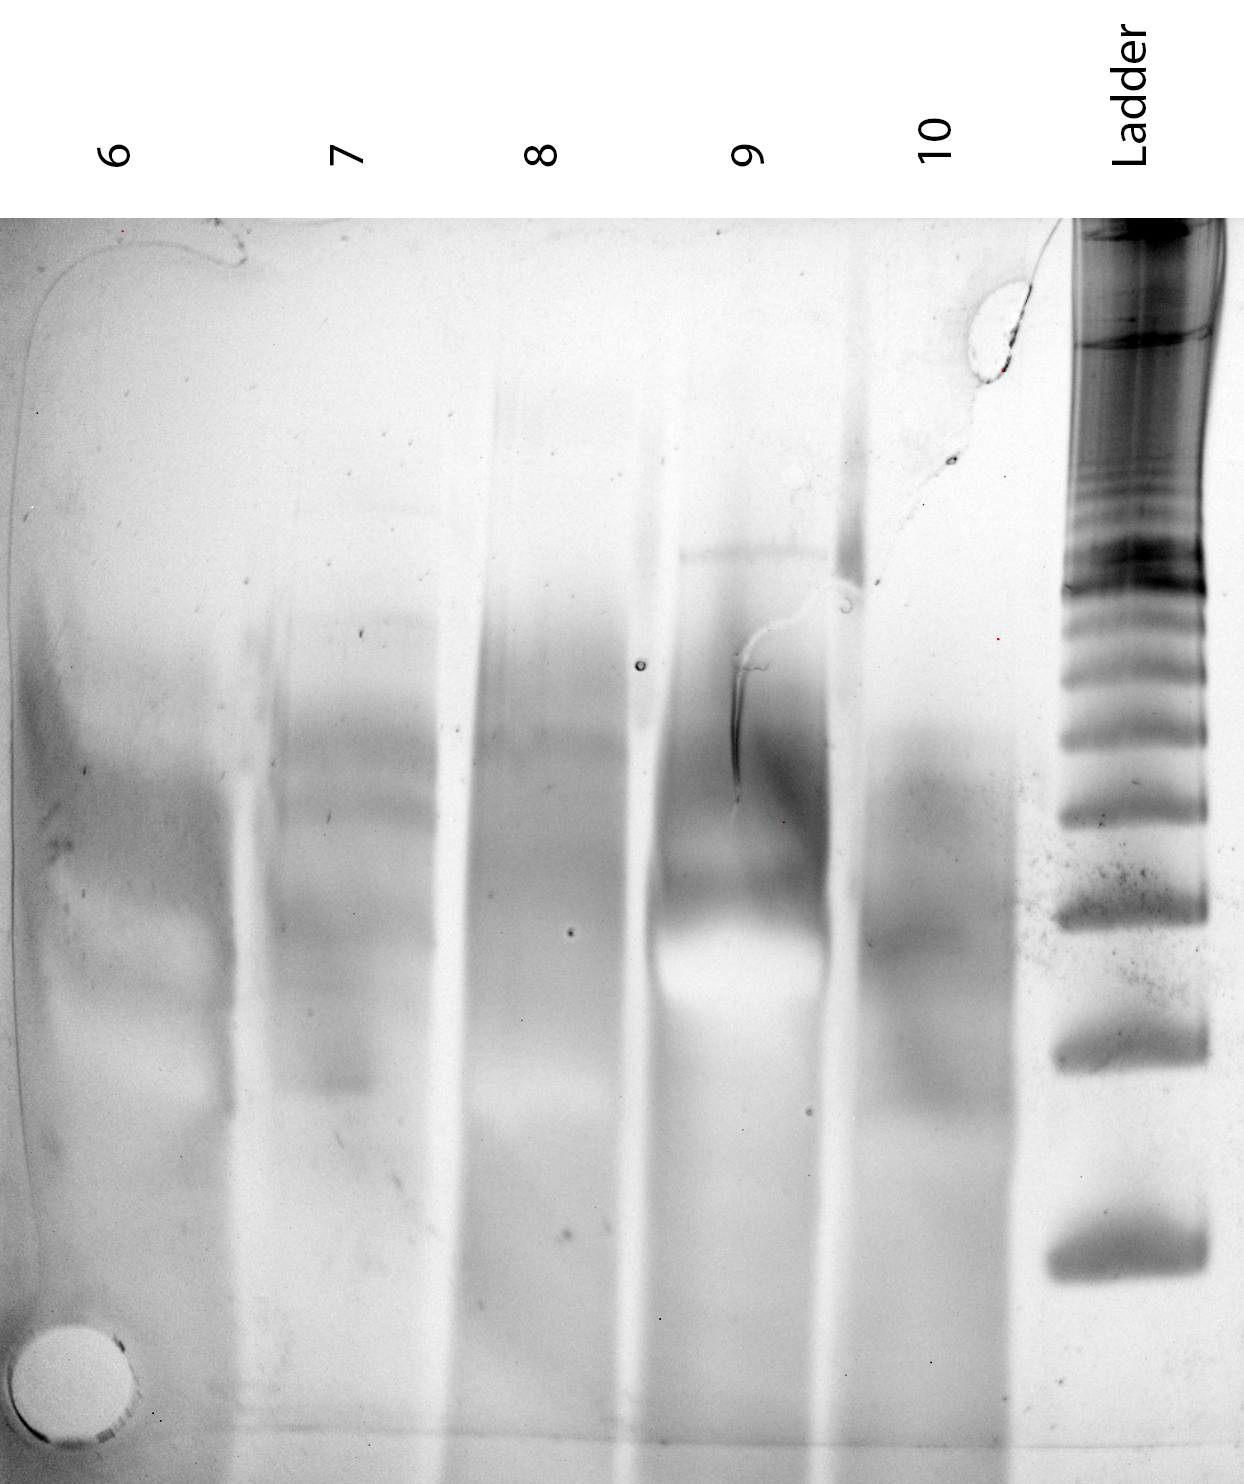
\includegraphics[width=150pt]{images/translator_transcription_long_2.png}
\caption{Transcription of the long translator sequences with a 10 nt ladder.}
\label{translator_transcription_long_2}
\end{figure}

Some of the other group members had previously had issues with running transcriptions on templates that was only partly double-stranded with the T7 promoter sequence. To get fully double-stranded templates, some reverse primers for the template strands was ordered from IDT, and the T7 promoter could be used as the forward primer. A PCR reaction was done (\tref{pcr}), run on a 2\% agarose SB at 300 V for 15 minutes, stained in SYBR Gold and scanned.

\begin{table}\centering
\begin{tabular}{llll}
  \hline
   & \textbf{Initial conc.} & \textbf{Final conc.} & \textbf{Volume} \\ \hline
  HF & 5X                    & 1X                   & 10 \si{\micro}L           \\
  Forward primer (T7 promoter)                 & 100 \si{\micro}M                 & 2 \si{\micro}M                & 1 \si{\micro}L           \\
  Reverse primer                & 100 \si{\micro}M                 & 2 \si{\micro}M                & 1 \si{\micro}L           \\
  dNTP mix              & 25 mM                  & 250 nM               & 0.5 \si{\micro}L           \\
  Template             & 1 \si{\micro}M                 & 10 nM                & 0.5 \si{\micro}L           \\
  Phusion polymerase    &                        &                      & 0.5 \si{\micro}L            \\
  Nuclease-free water  &                        &                      & 36 \si{\micro}L           \\
  Total                &                        &                      & 50 \si{\micro}L          \\ \hline
\end{tabular}
\caption{Mixing of compounds for the PCR reaction on the long translator sequences.}
\label{pcr}
\end{table}

\begin{figure}[H]
\centering
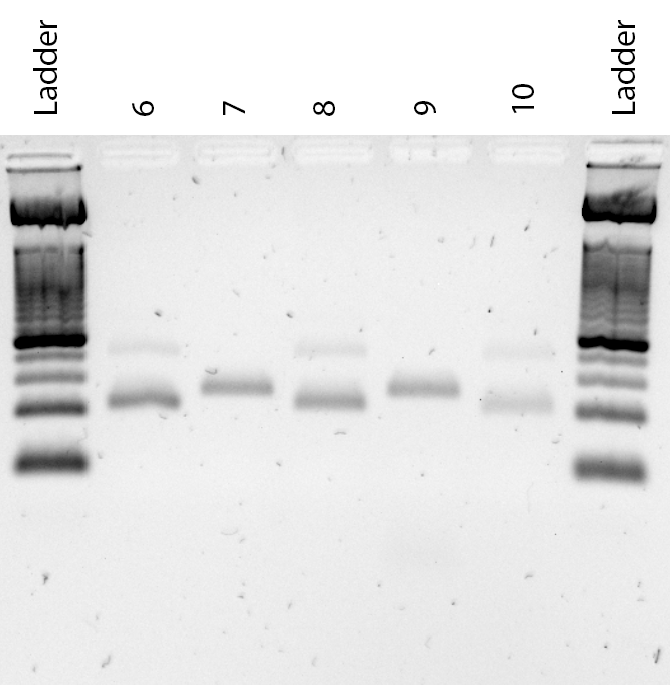
\includegraphics[width=150pt]{images/translator_pcr_long_1.png}
\caption{PCR product of the long translator sequences.}
\label{translator_pcr_long_1}
\end{figure}

The result in \fref{translator_pcr_long_1} shows the expected PCR product sizes compared with \tref{dna}. Another transcription reaction was carried out on the double-stranded long translator sequences using the previous protocol. The samples were run on a 10\% denaturing PAGE gel for 2 hours at 25 W. UV shadowing still only revealed a band in strand 10, so the gel was stained with SYBR Gold and scanned.

\begin{figure}[H]
\centering
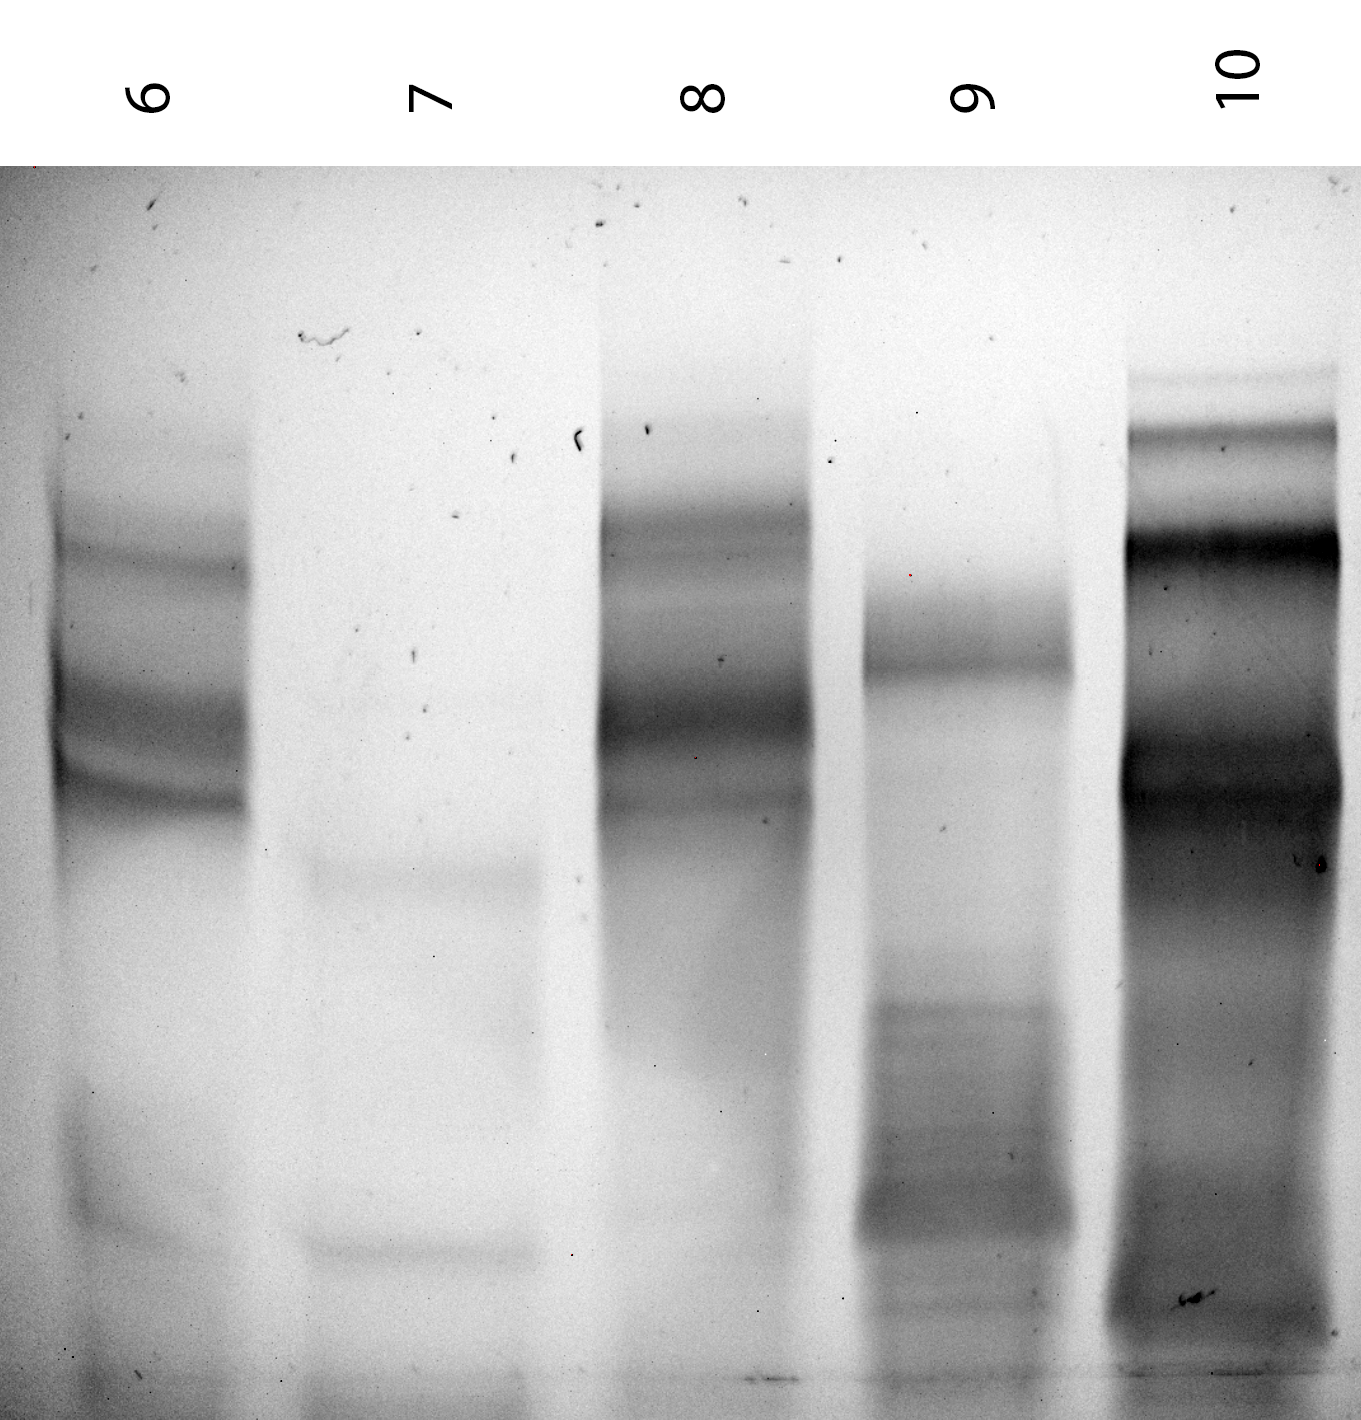
\includegraphics[width=150pt]{images/translator_transcription_long_ds_1.png}
\caption{Transcription of the double-stranded long translator sequences.}
\label{translator_transcription_long_ds_1}
\end{figure}

\fref{translator_transcription_long_ds_1} shows strand 10 clearly, but still a lot of other products, and strand 7 has hardly been transcribed at all. After some further discussion with the other group members, the results can be explained by secondary structures of the RNA strands. If the strands form strong hairpins, the transcription can be aborted early, and produce unintended products. The RNA strands were checked in Nupack for secondary structures. Comparing the Nupack analysis in \fref{long_secondary_structures} with the gel in \fref{translator_transcription_long_ds_1}, the amount of product seems to follow the free energy of the secondary structure of the RNA. Strand 10 which was visible in UV shadowing has no secondary structure with the highest probability, and and strand 7 which shows the least amount of product has the lowest free energy.

The only way to avoid this problem is to create another design which doesn't have secondary structures, but since the translator sequences are locked by the desired input and output sequences, this is not a possibility. To actually get the RNA strands, they should have been ordered from IDT, synthesized and purified. This is more expensive, and was thought to be unnecessary in the beginning of the experiment. There was not enough time left to order the RNA sequences and carry out the fluorescence measurements on the translator, so no results was obtained from the experiment.


  \chapter{Results and discussion}
  % !TEX root = ../main.tex

To test the perceptron compiling and training, 5 different truth tables were used, ranging from 2 to 3 inputs (\cref{2_and,2_or,3_and,3_1_or,3_2_or}). The correct output was reached after 16-23 iterations of the learning algorithm. Input sizes greater than 3 were not tested, as the training time increases exponentially in time with the input size. Only truth tables that didn't involve NOT and XOR logic were used, as no solutions exist to these problems with the current algorithm (no linear separability and negative weights).


\section{2-input AND}

\begin{figure}[H]
  \begin{subfigure}[t]{.49\columnwidth}

      \centering
    \begin{tabular}[b]{ccc}
      \hline
      \multicolumn{1}{l}{\textbf{Input 1}} & \multicolumn{1}{l}{\textbf{Input 2}} & \multicolumn{1}{l}{\textbf{Output}} \\
      \hline
      0                                    & 0                                    & 0                                   \\
      0                                    & 1                                    & 0                                   \\
      1                                    & 0                                    & 0                                   \\
      1                                    & 1                                    & 1 \\
      \hline
    \end{tabular}
    \caption{Truth table for the 2-input AND gate.}
  \end{subfigure}
  \begin{subfigure}[t]{.49\textwidth}
    \includegraphics[width=\textwidth]{figures/trained_2_and.tikz}
    \caption{Diagram of the 2-input AND with correct weights and threshold.}
  \end{subfigure}
\hfill
\begin{subfigure}[t]{\textwidth}
  \centering
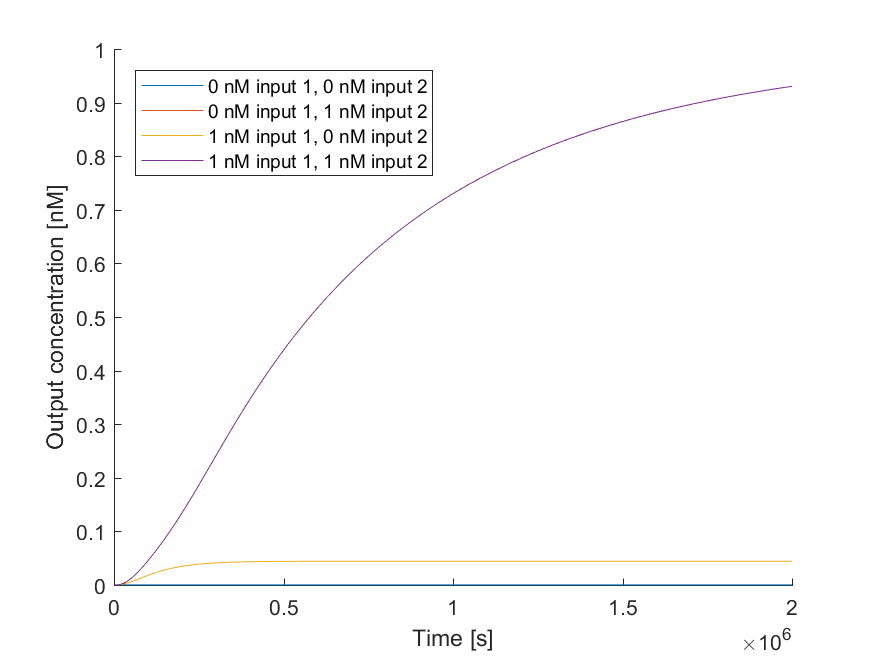
\includegraphics[width=\textwidth]{images/and_simulation.png}
\caption{Time analysis of the 2-input AND.}
\end{subfigure}
\caption{Simulation results of the trained 2-input AND gate. The network is trained to activate when both of the inputs are active. The correct output was obtained after 21 iterations of the training algorithm, with a weight of 1.9 for all inputs, and a threshold of 10.}
\label{2_and}
\end{figure}

\section{2-input OR}

\begin{figure}[H]
  \begin{subfigure}[t]{.49\columnwidth}

      \centering
    \begin{tabular}[b]{ccc}
      \hline
    \multicolumn{1}{l}{\textbf{Input 1}} & \multicolumn{1}{l}{\textbf{Input 2}} & \multicolumn{1}{l}{\textbf{Output}} \\
    \hline
    0                                    & 0                                    & 0                                   \\
    0                                    & 1                                    & 1                                   \\
    1                                    & 0                                    & 1                                   \\
    1                                    & 1                                    & 1 \\
    \hline
    \end{tabular}
    \caption{Truth table for the 2-input OR gate.}
\end{subfigure}
\begin{subfigure}[t]{.49\textwidth}
  \includegraphics[width=\textwidth]{figures/trained_2_or.tikz}
  \caption{Diagram of the 2-input OR with correct weights and threshold.}
\end{subfigure}
\hfill
\begin{subfigure}[t]{\textwidth}
  \centering
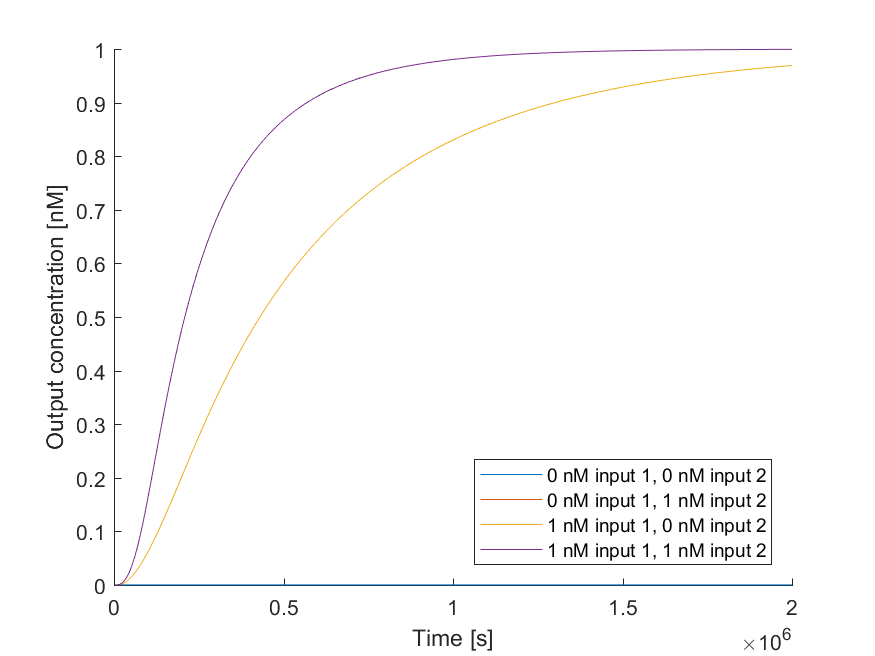
\includegraphics[width=\textwidth]{images/or_simulation.png}
\caption{Time analysis of the 2-input OR.}
\end{subfigure}
\caption{Simulation results of the trained 2-input OR gate. The network is trained to activate when one of the inputs is active. The correct output was obtained after 22 iterations of the training algorithm, with a weight of 2.1 for all inputs, and a threshold of 10.}
\label{2_or}
\end{figure}

\section{3-input AND}

\begin{figure}[H]
  \begin{subfigure}[t]{.49\columnwidth}
    \begin{adjustbox}{width=\textwidth}
    \begin{tabular}[b]{cccc}
      \hline
    \multicolumn{1}{l}{\textbf{Input 1}} & \multicolumn{1}{l}{\textbf{Input 2}} & \multicolumn{1}{l}{\textbf{Input 3}} & \multicolumn{1}{l}{\textbf{Output}} \\
    \hline
    0 & 0                                    & 0                                    & 0                                   \\
    0 & 0                                    & 1                                    & 0                                   \\
    0 & 1                                    & 0                                    & 0                                   \\
    0 & 1                                    & 1                                    & 0                                   \\
    1 & 0                                    & 0                                    & 0                                   \\
    1 & 0                                    & 1                                    & 0                                   \\
    1 & 1                                    & 0                                    & 0                                   \\
    1 & 1                                    & 1                                    & 1                                   \\

    \hline
    \end{tabular}
  \end{adjustbox}
    \caption{Truth table for the 3-input AND gate.}
\end{subfigure}
\begin{subfigure}[t]{.49\textwidth}
  \includegraphics[width=\textwidth]{figures/trained_3_and.tikz}
  \caption{Diagram of the 3-input AND with correct weights and threshold.}
\end{subfigure}
\hfill
\begin{subfigure}[t]{\textwidth}
  \centering
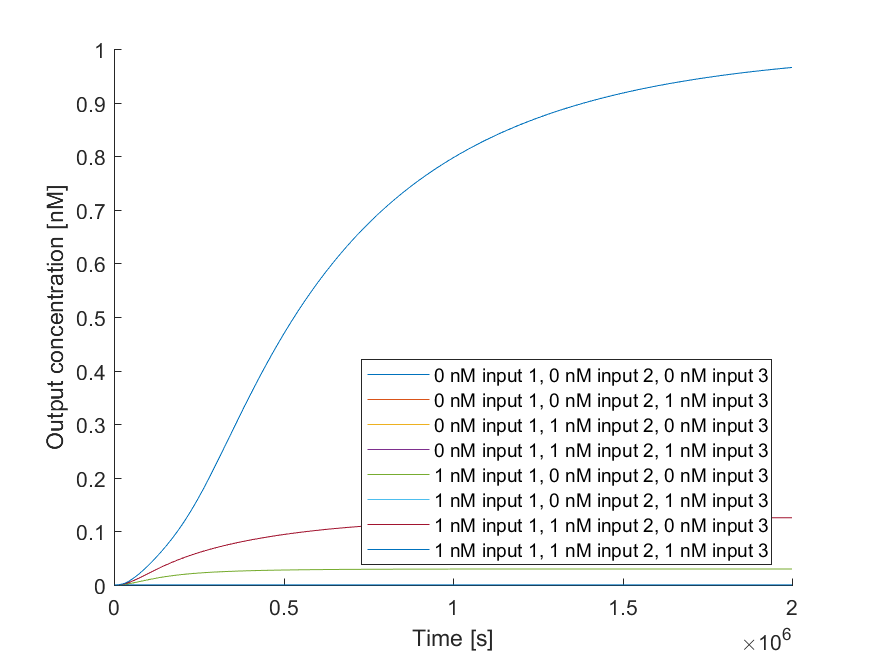
\includegraphics[width=\textwidth]{images/and_simulation_3input.png}
\caption{Time analysis of the 3-input AND.}
\end{subfigure}
\caption{Simulation results of the trained 3-input AND gate. The network is trained to activate when all of the inputs are active. The correct output was obtained after 14 iterations of the training algorithm, with a weight of 1.2 for all inputs, and a threshold of 10.}
\label{3_and}
\end{figure}

\section{3-input 1-OR}

\begin{figure}[H]
  \begin{subfigure}[t]{.49\columnwidth}

      \begin{adjustbox}{width=\textwidth}
    \begin{tabular}[b]{cccc}
      \hline
    \multicolumn{1}{l}{\textbf{Input 1}} & \multicolumn{1}{l}{\textbf{Input 2}} & \multicolumn{1}{l}{\textbf{Input 3}} & \multicolumn{1}{l}{\textbf{Output}} \\
    \hline
    0 & 0                                    & 0                                    & 0                                   \\
    0 & 0                                    & 1                                    & 1                                   \\
    0 & 1                                    & 0                                    & 1                                   \\
    0 & 1                                    & 1                                    & 1                                   \\
    1 & 0                                    & 0                                    & 1                                   \\
    1 & 0                                    & 1                                    & 1                                   \\
    1 & 1                                    & 0                                    & 1                                   \\
    1 & 1                                    & 1                                    & 1                                   \\

    \hline
    \end{tabular}
  \end{adjustbox}
    \caption{Truth table for the 3-input 1-OR gate.}
\end{subfigure}
\begin{subfigure}[t]{.49\textwidth}
  \includegraphics[width=\textwidth]{figures/trained_3_1_or.tikz}
  \caption{Diagram of the 3-input 1-OR with correct weights and threshold.}
\end{subfigure}
\hfill
\begin{subfigure}[t]{\textwidth}
  \centering
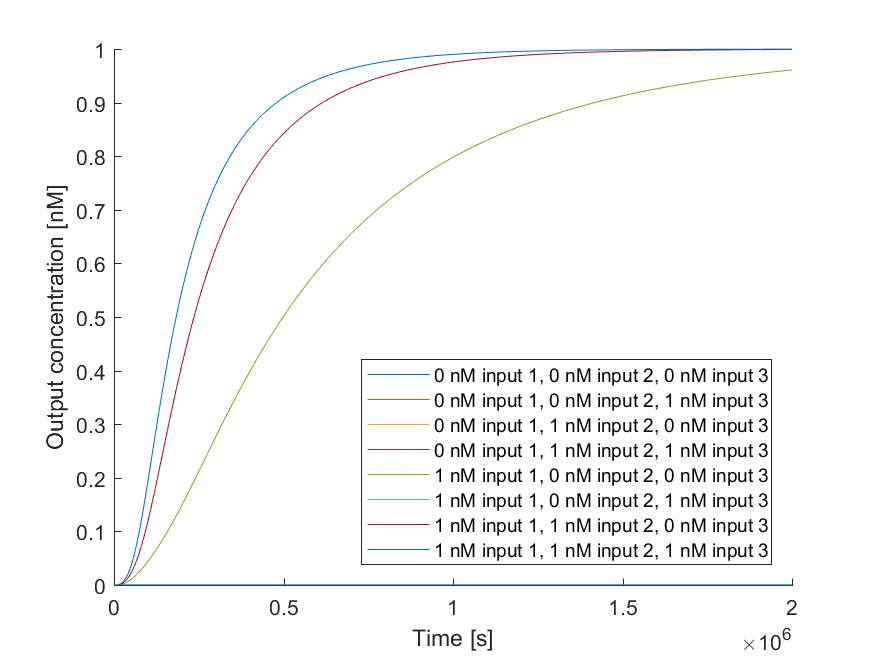
\includegraphics[width=\textwidth]{images/or_1_simulation_3input.png}
\caption{Time analysis of the 3-input 1-OR.}
\end{subfigure}
\caption{Simulation results of the trained 3-input 1-OR gate. The network is trained to activate when at least 1 of the inputs is active. The correct output was obtained after 16 iterations of the training algorithm, with a weight of 1.3 for all inputs, and a threshold of 10.}
\label{3_1_or}
\end{figure}

\section{3-input 2-OR}


\begin{figure}[H]
  \begin{subfigure}[t]{.49\columnwidth}
    \begin{adjustbox}{width=\textwidth}
    \begin{tabular}[b]{cccc}
      \hline
    \multicolumn{1}{l}{\textbf{Input 1}} & \multicolumn{1}{l}{\textbf{Input 2}} & \multicolumn{1}{l}{\textbf{Input 3}} & \multicolumn{1}{l}{\textbf{Output}} \\
    \hline
    0 & 0                                    & 0                                    & 0                                   \\
    0 & 0                                    & 1                                    & 0                                   \\
    0 & 1                                    & 0                                    & 0                                   \\
    0 & 1                                    & 1                                    & 1                                   \\
    1 & 0                                    & 0                                    & 0                                   \\
    1 & 0                                    & 1                                    & 1                                   \\
    1 & 1                                    & 0                                    & 1                                   \\
    1 & 1                                    & 1                                    & 1                                   \\

    \hline
    \end{tabular}
  \end{adjustbox}
    \caption{Truth table for the 3-input 2-OR gate.}
\end{subfigure}
\begin{subfigure}[t]{.49\textwidth}
  \includegraphics[width=\textwidth]{figures/trained_3_2_or.tikz}
  \caption{Diagram of the 3-input 2-OR with correct weights and threshold.}
\end{subfigure}
\hfill
\begin{subfigure}[t]{\textwidth}
  \centering
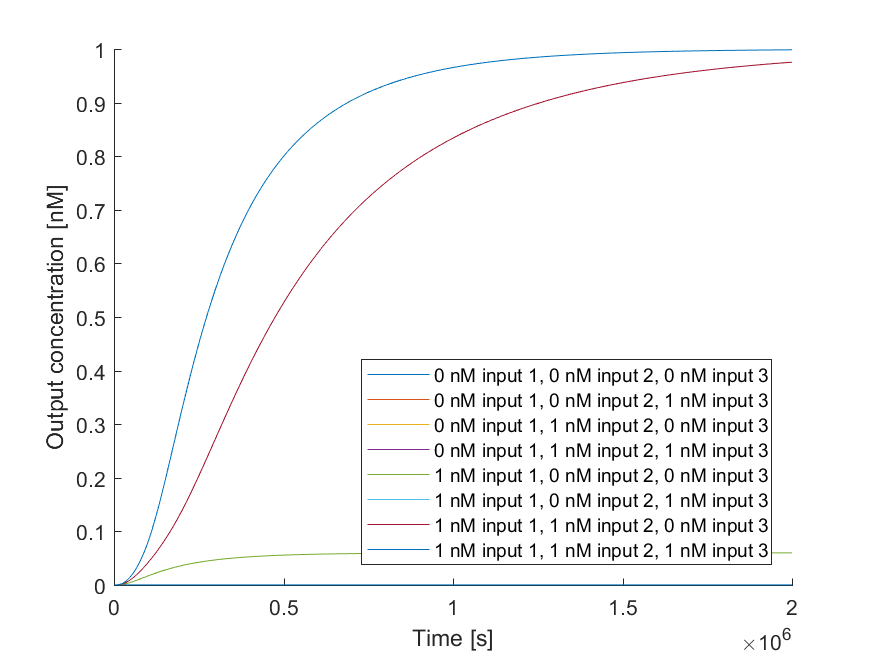
\includegraphics[width=\textwidth]{images/or_2_simulation_3input.png}
\caption{Time analysis of the 3-input 2-OR.}
\end{subfigure}
\caption{Simulation results of the trained 3-input 2-OR gate. The network is trained to activate when at least 2 of the inputs is active. The correct output was obtained after 15 iterations of the training algorithm, with a weight of 1.4 for all inputs, and a threshold of 10.}
\label{3_2_or}
\end{figure}



  \chapter{Conclusion}
  % !TEX root = ../main.tex

Since it was not possible to transcribe the RNA needed for testing the RNA translator, it is not possible to conclude anything from the results. The experiment was almost identical to the original article, and there is nothing to suggest that the strand displacement shouldn't have worked using RNA instead of DNA \cite{Picuri2009}. The original article even uses RNA as the input for the DNA translators.

The simulations of the neural network did show some promising results. It was possible to create multiple perceptrons of varying input size, and train them to different truth tables (\cref{2_and,2_or,3_and,3_1_or,3_2_or}). The system requires no input from the user after having defined the desired truth table.

The perceptron in this experiment is still only a stripped down version of the networks in the original article \cite{Qian2011}, as it was not possible to apply the dual-rail logic needed for avoiding negative weights. It was not possible to translate the input sequences using Nupack either. Furthermore, the perceptrons trained in this experiment, could have been made much simpler by the logic gate system the authors of the original article designed recently \cite{Thubagere2017}. The only novel thing that came out of this experiment was the simplified training algorithm for the perceptrons without dual-rail logic.

There is also the problem of applying the simulations to in vitro reactions. The original paper found some general guidelines for adjusting the concentrations that seemed to work for some networks, but it can't be expected that the sequences and concentrations found in the simulation will always work in vitro. In the original paper, they also express concern for moving to in vivo.

Still, the preliminary work done in this experiment could in theory be used to create a generic method for designing RNA/DNA detection kits. With some more work, the training algorithm and input translation could be combined, and tested in vitro.


  \bibliographystyle{unsrt}
  \bibliography{references}

  \appendix
  \chapter{Appendix}
  % !TEX root = ../main.tex
\begin{figure}[h]
\begin{subfigure}[b]{.49\columnwidth}
  \centering
  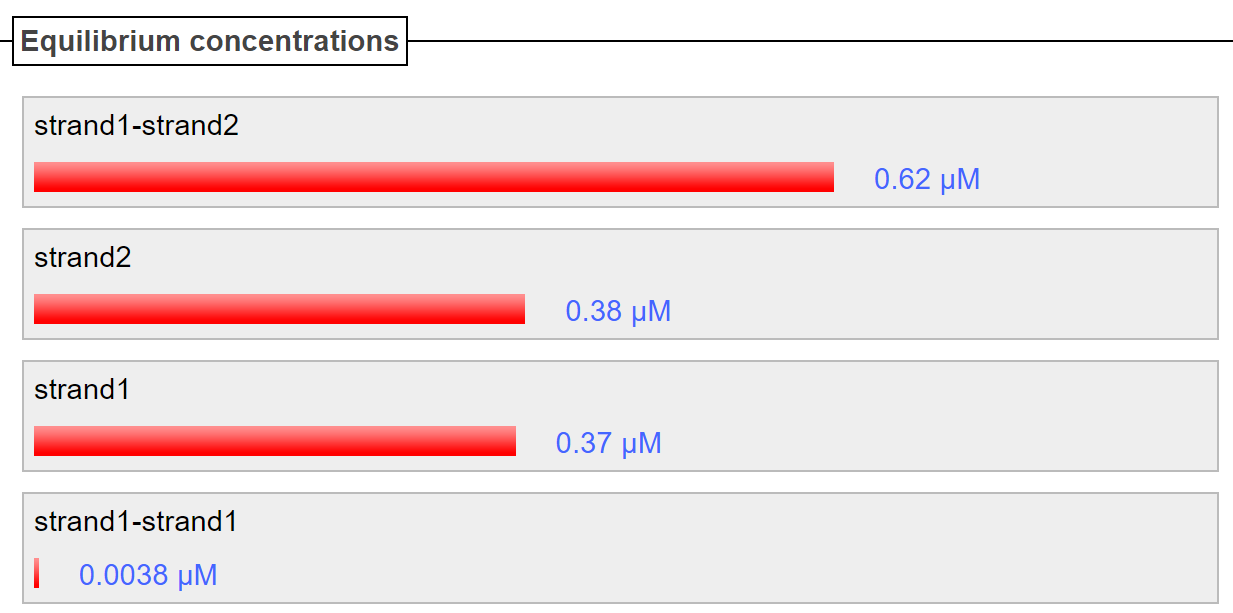
\includegraphics[width=\linewidth]{images/short_annealing_concentration.png}
  \caption{Equilibrium concentration of the short translator strands 1 and 2.}
\end{subfigure}
\hfill
\begin{subfigure}[b]{.49\columnwidth}
  \centering
  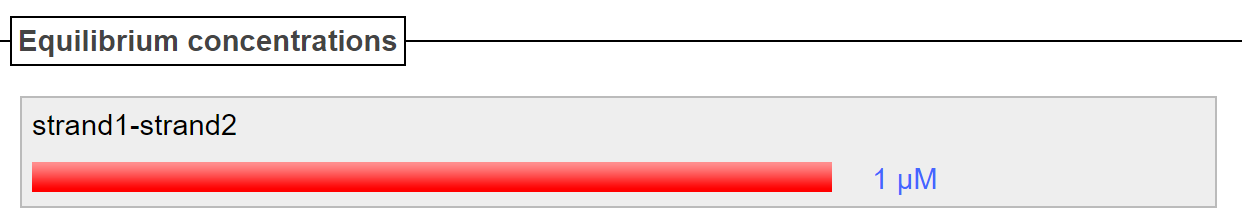
\includegraphics[width=\linewidth]{images/long_annealing_concentration.png}
  \caption{Equilibrium concentration of the long translator strands 6 and 7.}
\end{subfigure}
\caption{Nupack analysis of the equilibrium concentrations of the first subunit of the short and long translator.}
\label{annealing_concentration}
\end{figure}

\begin{figure}[h]
\centering
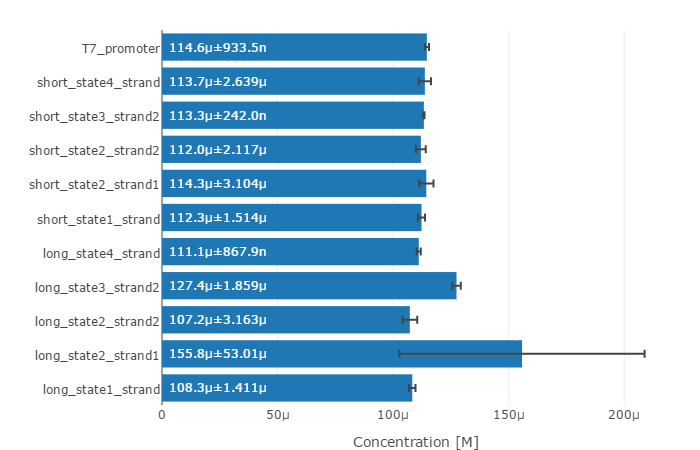
\includegraphics[width=\columnwidth]{images/oligo_concentrations.png}
\caption{Concentrations of the dissolved DNA oligos ordered from IDT.}
\label{oligo_concentrations}
\end{figure}

\begin{figure}[h]
\centering
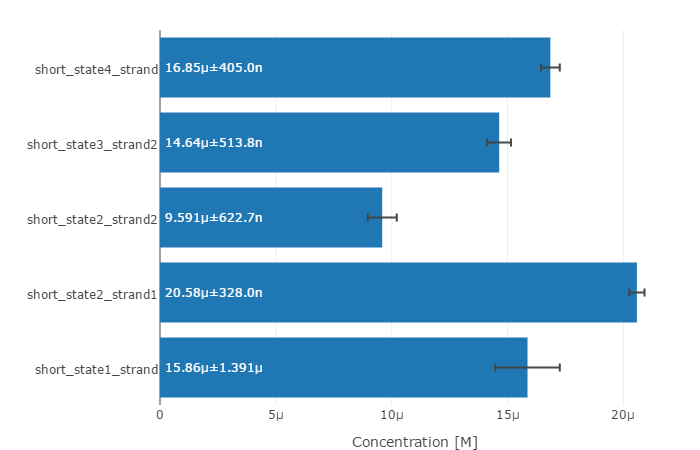
\includegraphics[width=\columnwidth]{images/translator_transcription_concentration.png}
\caption{Concentrations of the short translator RNA sequences.}
\label{translator_transcription_concentration}
\end{figure}


\begin{figure}[h]
\begin{subfigure}{.32\columnwidth}
  \centering
  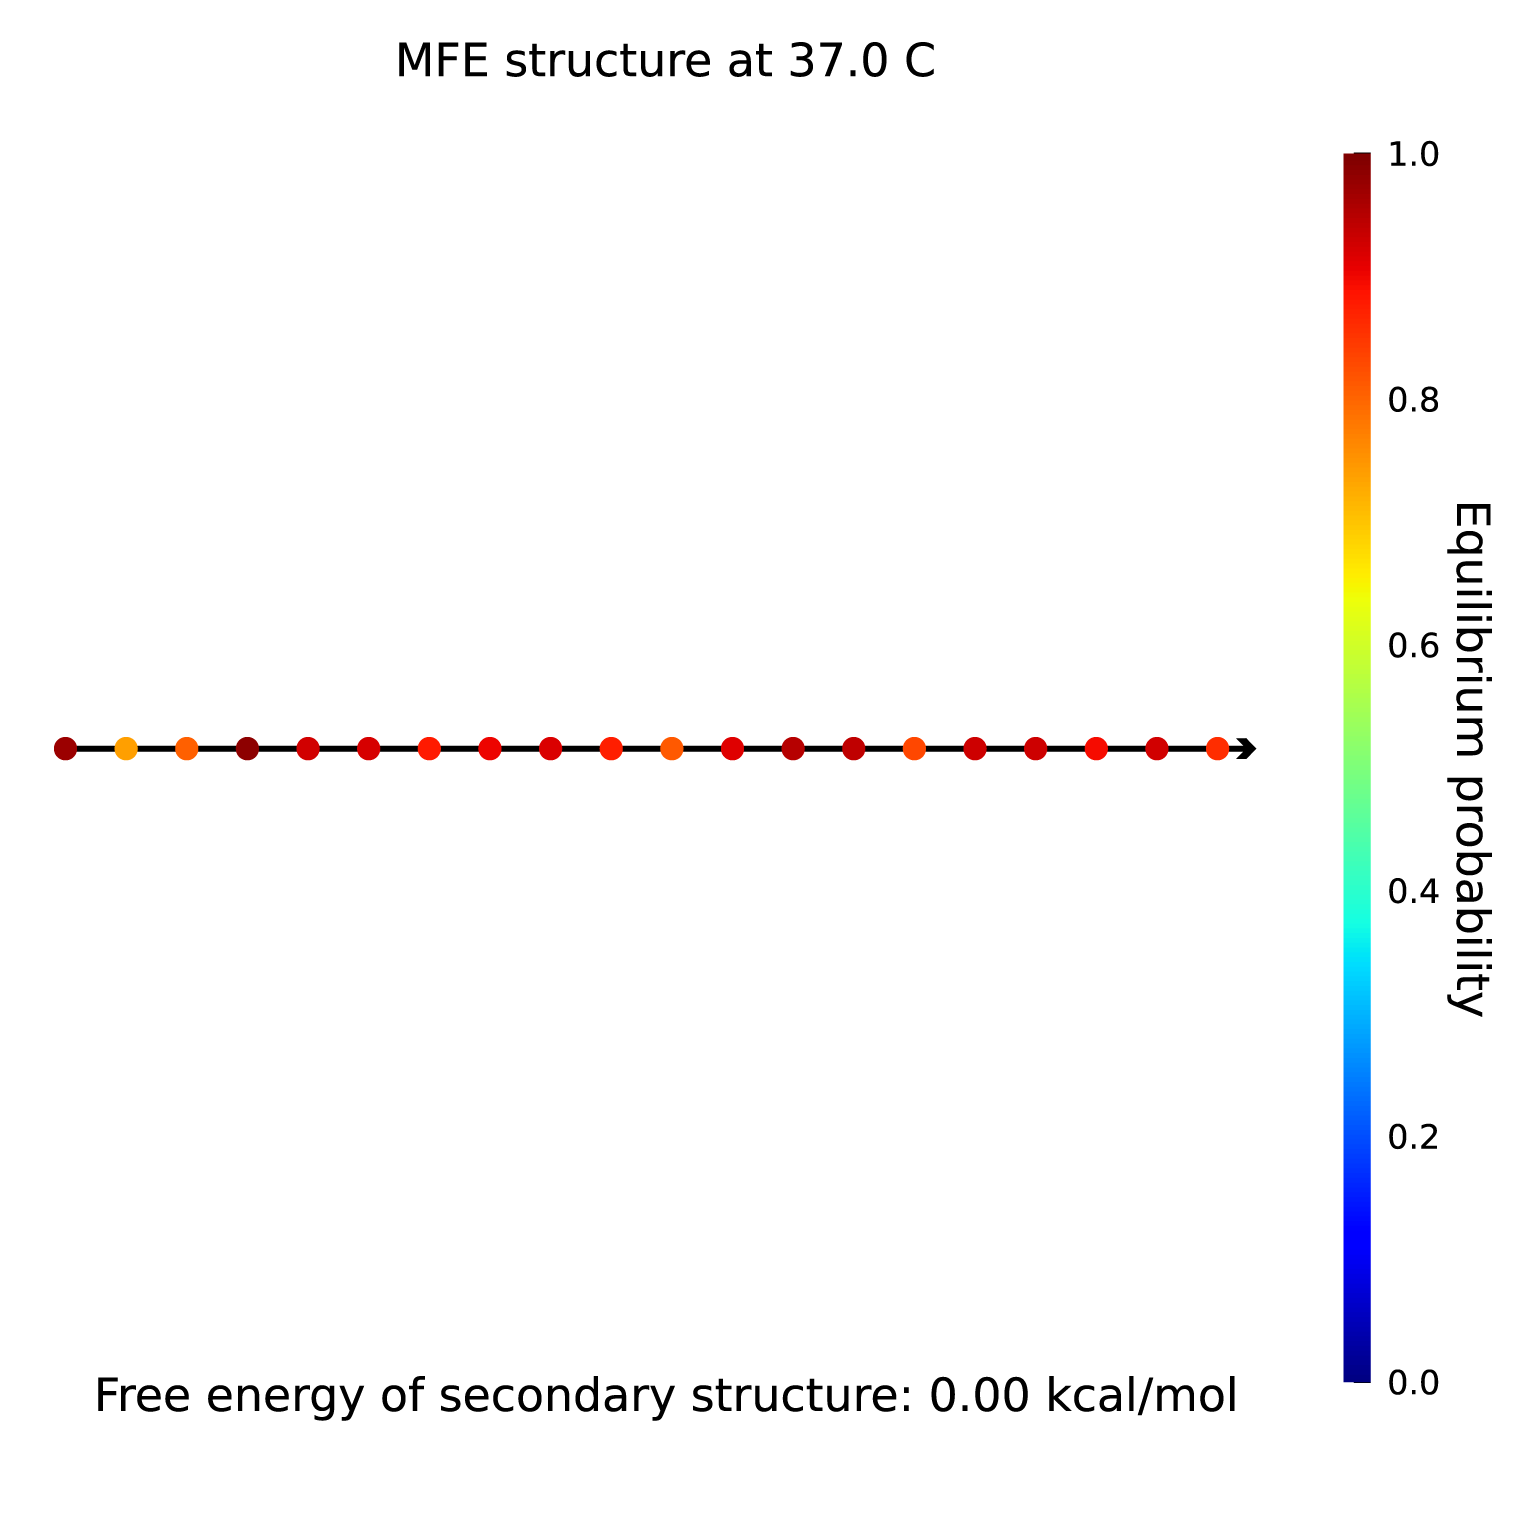
\includegraphics[width=\linewidth]{images/0_analysis.png}
  \caption{T7 promoter}
\end{subfigure}%
\begin{subfigure}{.32\columnwidth}
  \centering
  \includegraphics[width=\linewidth]{images/1_analysis.png}
  \caption{Short 1}
\end{subfigure}
\begin{subfigure}{.32\columnwidth}
  \centering
  \includegraphics[width=\linewidth]{images/2_analysis.png}
  \caption{Short 2}
\end{subfigure}
\begin{subfigure}{.32\columnwidth}
  \centering
  \includegraphics[width=\linewidth]{images/3_analysis.png}
  \caption{Short 3}
\end{subfigure}
\begin{subfigure}{.32\columnwidth}
  \centering
  \includegraphics[width=\linewidth]{images/4_analysis.png}
  \caption{Short 4}
\end{subfigure}
\begin{subfigure}{.32\columnwidth}
  \centering
  \includegraphics[width=\linewidth]{images/5_analysis.png}
  \caption{Short 5}
\end{subfigure}
\caption{Secondary structures of the DNA sequences for the short translator and the T7 promoter sequence.}
\label{short_secondary_structures}
\end{figure}

\begin{figure}[h]
\begin{subfigure}{.32\columnwidth}
  \centering
  \includegraphics[width=\linewidth]{images/long_rna_secondarystructure_6.png}
  \caption{Long 6}
\end{subfigure}%
\begin{subfigure}{.32\columnwidth}
  \centering
  \includegraphics[width=\linewidth]{images/long_rna_secondarystructure_7.png}
  \caption{Long 7}
\end{subfigure}
\begin{subfigure}{.32\columnwidth}
  \centering
  \includegraphics[width=\linewidth]{images/long_rna_secondarystructure_8.png}
  \caption{Long 8}
\end{subfigure}
\begin{subfigure}{.32\columnwidth}
  \centering
  \includegraphics[width=\linewidth]{images/long_rna_secondarystructure_9.png}
  \caption{Long 9}
\end{subfigure}
\begin{subfigure}{.32\columnwidth}
  \centering
  \includegraphics[width=\linewidth]{images/long_rna_secondarystructure_10.png}
  \caption{Long 10}
\end{subfigure}
\caption{Secondary structures of the RNA sequences for the long translator.}
\label{long_secondary_structures}
\end{figure}

\begin{table}[h]
\centering
\begin{tabular}{ll}
  \hline
\textbf{}           & \textbf{Concentration} \\
\hline
Tris-HCl pH 8.0     & 10 nM                  \\
EDTA                & 1 mM                   \\
Nuclease-free water &               \\
\hline
\end{tabular}
\caption{Contents of 1X TE buffer.}
\label{te_buffer}
\end{table}

\begin{table}[h]
\centering
\begin{tabular}{ll}
  \hline
\textbf{}           & \textbf{Concentration} \\
\hline
Tris pH 8.0     & 10 nM                  \\
NaCl                & 50 mM                   \\
EDTA                & 1 mM                   \\
Nuclease-free water &               \\
\hline
\end{tabular}
\caption{Contents of 1X annealing buffer.}
\label{annealing_buffer}
\end{table}

\begin{table}[h]
\centering
\begin{tabular}{ll}
  \hline
\textbf{}           & \textbf{Concentration} \\
\hline
Xylene cyanol     & 0.04\%                 \\
Bromophenol blue                & 0.04\%                   \\
Glycerol                & 20\%                   \\
Nuclease-free water &               \\
\hline
\end{tabular}
\caption{Contents of native loading buffer.}
\label{native_buffer}
\end{table}

\begin{table}[h]
\centering
\begin{tabular}{ll}
  \hline
\textbf{}           & \textbf{Concentration} \\
\hline
Xylene cyanol     & 0.04\%                 \\
Bromophenol blue                & 0.04\%                   \\
Glycerol                & 20\%                   \\
Urea & 5.4 M              \\
\hline
\end{tabular}
\caption{Contents of denaturing loading buffer.}
\label{denaturing_buffer}
\end{table}

\begin{lstlisting}[float,floatplacement=h,caption=Nupack code for the short translator, label=codeshort]
structure state1 = ......................
structure state2 = ............((((((((((+............))))))))))
structure state3 = .............((((((((((+............))))))))))
structure state4 = .......................

domain a = N10
domain b = N10
domain c = CUCCUUGAGG
domain d = CUAGACUGAAG
domain e = GG

state1.seq = e a b
state2.seq = e c a e b* a*
state3.seq = e d c e a* c*
state4.seq = e d c

prevent = AAAA, CCCC, GGGG, UUUU, KKKKKK, MMMMMM, RRRRRR, SSSSSS, WWWWWW, YYYYYY
\end{lstlisting}


\begin{lstlisting}[float,floatplacement=h, caption=Nupack code for the long translator, label=codelong]
structure state1 = ................................
structure state2 = ......................((((((((((((((((((((+............))))))))))))))))))))
structure state3 = ............((((((((((((((((((((+......................))))))))))))))))))))
structure state4 = ................................

domain a = N20
domain b = N10
domain c = GCUCCUUGAGG N9
domain d = CUAGACUGAA
domain e = GG

state1.seq = e a b
state2.seq = e c a e b* a*
state3.seq = e d c e a* c*
state4.seq = e d c

prevent = AAAA, CCCC, GGGG, UUUU, KKKKKK, MMMMMM, RRRRRR, SSSSSS, WWWWWW, YYYYYY
\end{lstlisting}


\end{document}
